\documentclass[12pt,a4paper]{article}
\usepackage[left=1.5cm,right=1.5cm,top=2cm,bottom=2cm]{geometry}
% \usepackage[margin=2.5cm]{geometry}
\usepackage{setspace}\onehalfspacing
\usepackage{graphicx,float,caption,subcaption}
\usepackage{booktabs,array,tabularx}
\usepackage{amsmath,amssymb}
\usepackage{xcolor}
\usepackage{listings}
\usepackage{pgfplots}\pgfplotsset{compat=1.17}
\usepackage{tikz}
\usepackage{fancyhdr}
\usepackage{longtable}
\usepackage{indentfirst}
\usepackage{xurl}
\usepackage[hidelinks]{hyperref}

\definecolor{aupp}{HTML}{1F2A5C}
\definecolor{codebg}{HTML}{F8F8F8}
\definecolor{pykw}{HTML}{0000CC}
\definecolor{pystr}{HTML}{B22222}
\definecolor{pycom}{HTML}{228B22}
\definecolor{pynum}{HTML}{FF8C00}
\definecolor{pybuiltin}{HTML}{7B2D8E}
\lstdefinestyle{pystyle}{
  language=Python,
  basicstyle=\ttfamily\footnotesize,
  backgroundcolor=\color{codebg},
  keywordstyle=\color{pykw}\bfseries,
  keywordstyle=[2]\color{pybuiltin},
  stringstyle=\color{pystr},
  commentstyle=\color{pycom}\itshape,
  numberstyle=\tiny\color{gray},
  numbers=left, numbersep=6pt,
  frame=single, rulecolor=\color{lightgray},
  breaklines=true, showstringspaces=false,
  morekeywords=[2]{print,len,range,dict,list,set,int,float,str,self,True,False,None},
  literate=*{0}{{{\color{pynum}0}}}1 {1}{{{\color{pynum}1}}}1 {2}{{{\color{pynum}2}}}1
            {3}{{{\color{pynum}3}}}1 {4}{{{\color{pynum}4}}}1 {5}{{{\color{pynum}5}}}1
            {6}{{{\color{pynum}6}}}1 {7}{{{\color{pynum}7}}}1 {8}{{{\color{pynum}8}}}1
            {9}{{{\color{pynum}9}}}1
}
\lstset{style=pystyle}

\pagestyle{fancy}\fancyhf{}
\lhead{American University of Phnom Penh}\rhead{Data Analysis I (Final Project Report)}
\lfoot{KHOV Seangngy \& PHAUT Sovannvatanak}\rfoot{Lecturer: Dr. HAS Sothea}
\cfoot{\thepage}
\renewcommand{\footrulewidth}{0.4pt}

\begin{document}
%==================== COVER ====================
\pagenumbering{gobble}
\begin{titlepage}
\centering
\parbox[c][2cm][c]{6cm}{\centering{
\includegraphics[scale=.7]{logo.png}}}\\[2.5cm]
{\Huge\bfseries\color{aupp} What Drives Life Expectancy?\\[0.3cm]
\Large A Regression Analysis of WHO Country-Level Health Data\par}
\vspace{2cm}
{\large\textbf{Course:} Data Analysis I\\[4pt]
\textbf{Lecturer:} Dr.\ HAS Sothea\\[4pt]
\textbf{Semester:} Fall 2027}\\[1.5cm]
{\large\textbf{Team Members}\\[4pt]
KHOV Seangngy (2026571) \\
PHAUT Sovannvatanak (2026525) }\\[1.5cm]
\textbf{Date:} November 28, 2026
\vfill
\end{titlepage}

\clearpage
\pagenumbering{roman}\setcounter{page}{1}
\pagestyle{plain}
{\singlespacing\tableofcontents}
\clearpage
\setlength{\headheight}{15pt}
\pagestyle{fancy}
\pagenumbering{arabic}\setcounter{page}{1}

%==================== I. INTRODUCTION ====================
\section{Introduction}
\subsection{Overview}
Life expectancy at birth is one of the most widely used indicators of a country's overall health and development. It reflects not only the quality of healthcare, but also education, income, nutrition, and disease burden. Understanding which of these factors matter most helps governments and health organizations decide where to invest limited resources. This project analyzes the Life Expectancy (WHO) dataset from Kaggle, which combines health and socioeconomic indicators for about 190 countries from 2000 to 2015. The data contains both quantitative variables (such as adult mortality, immunization coverage, GDP, and schooling) and qualitative variables (such as country and development status). It also contains missing and invalid values, so careful cleaning is required before modeling. Using a data analysis pipeline of preprocessing, exploratory analysis, regression modeling, and evaluation, we identify the strongest drivers of life expectancy and assess how accurately it can be predicted.

\subsection{Objective}
The primary objective of this project is to build and evaluate regression models
that predict a country's life expectancy from health, economic and social
indicators, and to identify which factors have the strongest influence.

The specific objectives are:
\begin{enumerate}
  \item Clean and preprocess the data by handling missing values, invalid
        values, outliers and inconsistent column names.
  \item Explore the relationships between life expectancy and the other
        variables using statistical summaries, visualizations and correlation
        analysis.
  \item Develop and compare several regression models against a baseline using
        RMSE, MAE and $R^2$.
  \item Interpret the best model to determine the main drivers of life
        expectancy and discuss their practical implications.
\end{enumerate}

\subsection{Dataset Summary}
\begin{table}[H]\centering
\caption{Dataset overview.}
\begin{tabularx}{\textwidth}{lX}\toprule
\textbf{Item} & \textbf{Description}\\\midrule
Source & Kaggle -- Life Expectancy (WHO) (Kumar Rajarshi), compiled from WHO and United Nations data. \url{https://www.kaggle.com/datasets/kumarajarshi/life-expectancy-who}\\
Coverage & 193 countries, 2000--2015 (183 countries remain after cleaning); one row per country per year\\
Size & 2938 rows $\times$ 22 columns (raw); 2928 rows $\times$ 24 columns (after cleaned, with 2 additional columns engineered for EDA)\\
Target & \texttt{life\_expectancy} (years)\\
Quantitative & 18 numeric predictors (plus target \texttt{life\_expectancy}), e.g.\ \texttt{adult\_mortality}, \texttt{bmi}, \texttt{gdp}, \texttt{schooling}\\
Qualitative & \texttt{country}, \texttt{status} (Developed/Developing); \texttt{year} is ordinal; engineered: \texttt{period}, \texttt{income\_tier}\\
Data quality issues & Missing values in 14 columns, implausible values (e.g.\ \texttt{bmi}, \texttt{measles}), inconsistent column names\\
Task & Supervised regression\\\bottomrule
\end{tabularx}
\end{table}

%==================== II. PREPROCESSING ====================
\section{Data Preprocessing}
\subsection{Initial Inspection}
The dataset was loaded with \texttt{pandas} from \texttt{Life Expectancy Data.csv}.
It contains \textbf{2938 rows and 22 columns} covering 193 countries from 2000 to 2015.
Key observations from the inspection:
\begin{itemize}
  \item \textbf{Column names:} several names contained trailing or repeated
        spaces (for example \texttt{"Life expectancy "}), so all names were
        stripped and converted to snake\_case.
  \item \textbf{Data types:} 20 columns are numeric (\texttt{float64}/\texttt{int64}) and
        2 are categorical (\texttt{object}/\texttt{str}): \texttt{country} and \texttt{status}.
  \item \textbf{Target variable:} \texttt{life\_expectancy} has a mean of 69.225 years,
        a standard deviation of 9.524, and ranges from 36.3 to 89.
  \item \textbf{Suspicious values:} the summary statistics show implausible
        values in several columns: \texttt{bmi} ranges from 1 to 87.3 (unrealistic
        for a national average), \texttt{adult\_mortality} has a minimum of 1,
        \texttt{measles} reaches 212,183 although it is reported per 1000
        population, \texttt{percentage\_expenditure} reaches 19,480 although it is
        a percentage, \texttt{population} has a minimum of 34, and \\
        \texttt{income\_composition\_of\_resources} and \texttt{schooling} have
        minimum values of 0. These are handled in
        Section~\ref{sec:invalid}.
  \item \textbf{Missing values:} 14 of the 22 columns contain missing values.
        The highest rates are \texttt{population} (22.19\%),
        \texttt{hepatitis\_b} (18.82\%) and \texttt{gdp} (15.25\%), examined in
        the next subsection. No duplicate rows were found.
\end{itemize}

\begin{lstlisting}
data = pd.read_csv("Life Expectancy Data.csv")
print(data.shape)

data.columns = (data.columns.str.strip().str.lower()
                .str.replace(r"[\s\-/]+", "_", regex=True))
data.info()
data.describe().T
\end{lstlisting}

\begin{table}[H]\centering
\caption{Summary statistics of all numeric features (before cleaning).}
\resizebox{\textwidth}{!}{%
\begin{tabular}{lrrrrrr}\toprule
\textbf{Feature} & \textbf{Count} & \textbf{Mean} & \textbf{Std} & \textbf{Min} & \textbf{Median} & \textbf{Max}\\\midrule
year & 2938 & 2007.52 & 4.61 & 2000 & 2008 & 2015\\
life\_expectancy & 2928 & 69.22 & 9.52 & 36.3 & 72.1 & 89.0\\
adult\_mortality & 2928 & 164.80 & 124.29 & 1 & 144 & 723\\
infant\_deaths & 2938 & 30.30 & 117.93 & 0 & 3 & 1800\\
alcohol & 2744 & 4.60 & 4.05 & 0.01 & 3.76 & 17.87\\
percentage\_expenditure & 2938 & 738.25 & 1987.91 & 0 & 64.91 & 19479.91\\
hepatitis\_b & 2385 & 80.94 & 25.07 & 1 & 92 & 99\\
measles & 2938 & 2419.59 & 11467.27 & 0 & 17 & 212183\\
bmi & 2904 & 38.32 & 20.04 & 1 & 43.5 & 87.3\\
under\_five\_deaths & 2938 & 42.04 & 160.45 & 0 & 4 & 2500\\
polio & 2919 & 82.55 & 23.43 & 3 & 93 & 99\\
total\_expenditure & 2712 & 5.94 & 2.50 & 0.37 & 5.76 & 17.6\\
diphtheria & 2919 & 82.32 & 23.72 & 2 & 93 & 99\\
hiv\_aids & 2938 & 1.74 & 5.08 & 0.1 & 0.1 & 50.6\\
gdp & 2490 & 7483.16 & 14270.17 & 1.68 & 1766.95 & 119172.7\\
population & 2286 & $1.28\times10^{7}$ & $6.10\times10^{7}$ & 34 & $1.39\times10^{6}$ & $1.29\times10^{9}$\\
thinness\_1\_19\_years & 2904 & 4.84 & 4.42 & 0.1 & 3.3 & 27.7\\
thinness\_5\_9\_years & 2904 & 4.87 & 4.51 & 0.1 & 3.3 & 28.6\\
income\_composition\_of\_resources & 2771 & 0.628 & 0.211 & 0 & 0.677 & 0.948\\
schooling & 2775 & 11.99 & 3.36 & 0 & 12.3 & 20.7\\\bottomrule
\end{tabular}}
\end{table}

\subsection{Duplicates}
A check for duplicate rows was performed using \texttt{duplicated()}. The result
confirmed that \textbf{no duplicate rows} exist in the dataset (0 duplicates found).
Since each row should represent one country in one year, we also checked
that the \texttt{(country, year)} pairs are unique. Therefore, no rows were removed.

%\begin{lstlisting}
%print(data.duplicated().sum())                              # 0
%print(data.duplicated(subset=["country", "year"]).sum())    # 0
%\end{lstlisting}

\subsection{Missing Values}
14 of the 22 columns contain missing values. The most affected columns are
\texttt{population} (22.19\%), \texttt{hepatitis\_b} (18.82\%) and \texttt{gdp}
(15.25\%), while the target \texttt{life\_expectancy} is missing in only 10 rows (0.34\%).

\begin{table}[H]\centering
\caption{Missing values per column ($n$ = 2938).}
\begin{tabular}{lrr}\toprule
\textbf{Column} & \textbf{Missing ($n$)} & \textbf{Missing (\%)}\\\midrule
population & 652 & 22.19\\
hepatitis\_b & 553 & 18.82\\
gdp & 448 & 15.25\\
total\_expenditure & 226 & 7.69\\
alcohol & 194 & 6.60\\
income\_composition\_of\_resources & 167 & 5.68\\
schooling & 163 & 5.55\\
bmi & 34 & 1.16\\
thinness\_1\_19\_years & 34 & 1.16\\
thinness\_5\_9\_years & 34 & 1.16\\
polio & 19 & 0.65\\
diphtheria & 19 & 0.65\\
life\_expectancy & 10 & 0.34\\
adult\_mortality & 10 & 0.34\\\bottomrule
\end{tabular}\end{table}

\begin{figure}[H]\centering
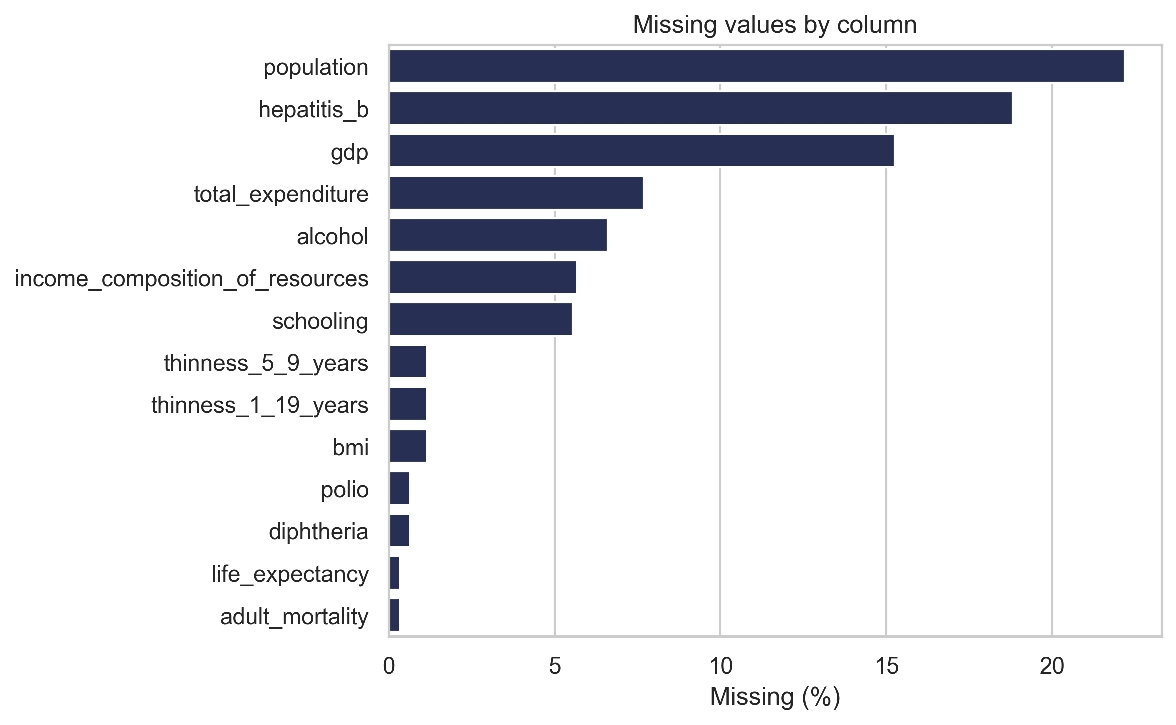
\includegraphics[width=0.85\textwidth]{figs/missing_values_bar.pdf}
\caption{Percentage of missing values by column.}
\end{figure}

\textbf{Pattern of missingness.} The missing values are not spread randomly:
\begin{itemize}
  \item \texttt{population}: 48 of the 49 affected countries are missing in \emph{all}
        16 years, so entire countries are absent from the source.
  \item \texttt{gdp}: 30 of the 38 affected countries are missing in all years.
  \item \texttt{hepatitis\_b}: the number of missing rows falls steadily from 98 in 2000
        to 9 in 2015, and the missing rate is higher for Developed (33.8\%) than for
        Developing (15.7\%) countries.
\end{itemize}
Because missingness depends on observed variables (country, year and status), the data is
treated as Missing At Random (MAR) rather than Missing Completely At Random (MCAR).
The 10 rows with missing \texttt{life\_expectancy} are exactly the 10 rows with missing
\texttt{adult\_mortality}.

\textbf{Handling strategy.}
\begin{itemize}
  \item \textbf{Target variable:} the 10 rows with missing
        \texttt{life\_expectancy} were dropped, since imputing the target would
        bias the model.
  \item \textbf{Predictors:} missing values were imputed with the median of the
        same \texttt{country}, which preserves country-level differences.
        If a country had no observed value at all, the median of its
        \texttt{status} group (Developed or Developing) was used instead.
  \item \textbf{Why the median:} many of these variables are skewed
        (e.g.\ \texttt{gdp}, \texttt{population}, \texttt{hepatitis\_b}), so the median is
        more robust than the mean.
  \item \textbf{Limitation:} for countries missing a variable in every year
        (48 for \texttt{population}, 30 for \texttt{gdp}) the country median does not exist,
        so the status median is used, which is a cruder estimate.
\end{itemize}

\begin{lstlisting}
data = data.dropna(subset=["life_expectancy"]).reset_index(drop=True)
# invalid values are set to NaN first (Section 2.4)

num_cols = data.select_dtypes("number").columns.drop(["life_expectancy", "year"])
for col in num_cols:
    data[col] = data.groupby("country")[col].transform(lambda s: s.fillna(s.median()))
    data[col] = data.groupby("status")[col].transform(lambda s: s.fillna(s.median()))

print(data.isnull().sum().sum())   # 0
\end{lstlisting}
Imputation was applied after the invalid values in Section~\ref{sec:invalid} were set to
missing, so those values were imputed as well. After imputation, no missing values remained
in the dataset (2928 rows).

\subsection{Invalid Data}\label{sec:invalid}
\begin{table}[H]\centering\caption{Invalid-value rules and rows flagged ($n = 2928$).}
\begin{tabularx}{\textwidth}{Xrl}\toprule
\textbf{Rule} & \textbf{Rows} & \textbf{Action}\\\midrule
bmi outside 10--60 & 629 & set to NaN, impute\\
schooling = 0 & 26 & set to NaN, impute\\
income\_composition\_of\_resources = 0 & 130 & set to NaN, impute\\
population $<$ 1000 & 30 & set to NaN, impute\\
infant\_deaths = 0 with population $>$ 1M & 174 & set to NaN, impute\\
under\_five\_deaths = 0 with population $>$ 1M & 151 & set to NaN, impute\\
under\_five\_deaths $<$ infant\_deaths & 0 & flag only\\
measles $>$ 1000 (said to be per 1000) & 525 & flag only, log-transform\\
percentage\_expenditure $>$ 100 & 1301 & flag only, log-transform\\
adult\_mortality $<$ 10 & 86 & flag only\\
immunization coverage $>$ 100 & 0 & none\\\bottomrule
\end{tabularx}\end{table}

\texttt{bmi} is the most problematic variable: 629 rows (21.5\%) fall outside a plausible
range, and its mean of 38.3 is unrealistic for national averages. Even after cleaning,
it should be interpreted with caution.

\subsection{Outliers}
The IQR method (1.5$\times$IQR) flagged many observations in right-skewed variables:
\texttt{measles} (542 rows, 18.5\%), \texttt{hiv\_aids} (542, 18.5\%),
\texttt{gdp} (459, 15.7\%), \texttt{population} (452, 15.4\%),
\texttt{under\_five\_deaths} (394, 13.5\%), \texttt{percentage\_expenditure}
(388, 13.3\%) and \texttt{infant\_deaths} (315, 10.8\%). The target has only 10 outliers (0.3\%),
and \texttt{bmi} and \texttt{income\_composition\_of\_resources} have none.
These values are genuine (large countries, epidemics, wealthy economies), so none were removed.
Instead, features with skewness above 1.5 were log-transformed with $\log(1+x)$ before modeling.
Boxplots of all numeric features are shown in Figure~\ref{fig:boxplots} (Appendix~C).

\begin{table}[H]\centering
\caption{Skewness before and after the $\log(1+x)$ transform (features with skewness $>$ 1.5).}\label{tab:skew}
\begin{tabular}{lrr}\toprule
\textbf{Feature} & \textbf{Before} & \textbf{After}\\\midrule
population & 17.94 & $-0.37$\\
infant\_deaths & 9.77 & 0.70\\
under\_five\_deaths & 9.48 & 0.65\\
measles & 9.43 & 0.55\\
hiv\_aids & 5.39 & 2.12\\
percentage\_expenditure & 4.64 & $-0.08$\\
gdp & 3.46 & $-0.10$\\
thinness\_5\_9\_years & 1.79 & 0.10\\
thinness\_1\_19\_years & 1.72 & 0.13\\\bottomrule
\end{tabular}\end{table}

The transform brought eight of the nine features close to symmetric (all within $\pm$0.70).
\texttt{hiv\_aids} remains right-skewed (2.12) because most countries share the
minimum value of 0.1. Left-skewed features such as \texttt{hepatitis\_b}, \texttt{polio}
and \texttt{diphtheria} were not transformed, since a log transform would worsen their skew.
\texttt{under\_five\_deaths} and \texttt{thinness\_5\_9\_years} are transformed but later
excluded from the model because of multicollinearity (Section~\ref{sec:model}).

\subsection{Feature Engineering and Encoding}
Two categorical features were engineered for the exploratory analysis:
\begin{itemize}
  \item \texttt{period}: \texttt{year} grouped into 2000--04, 2005--09 and 2010--15.
  \item \texttt{income\_tier}: \texttt{gdp} split into three equal-sized groups
        (Low: up to \$945, Medium: \$947--\$3,737, High: above \$3,737 per capita).
\end{itemize}
For modeling, \texttt{status} was encoded as a binary variable (Developing = 0, Developed = 1),
and the nine skewed features listed in Table~\ref{tab:skew} were log-transformed.
\texttt{period} and \texttt{income\_tier} were not used as model inputs because they
are derived from \texttt{year} and \texttt{gdp}, and \texttt{country} was used only to
group the train/test split. Including the two engineered features, the final cleaned dataset has
2928 rows and 24 columns (22 after cleaning + 2 engineered for EDA).

%==================== III. EDA ====================
\section{Exploratory Data Analysis (EDA)}
\subsection{Univariate Analysis}
\begin{figure}[H]\centering
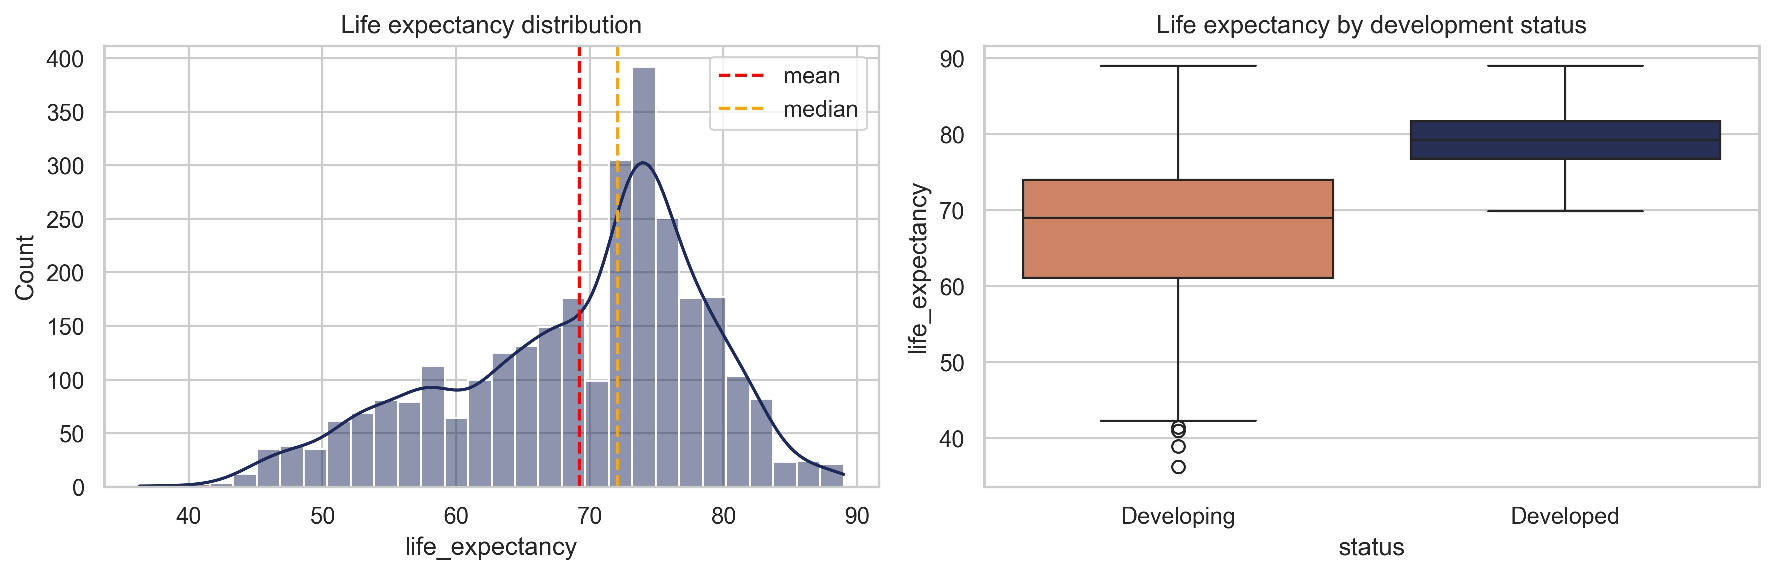
\includegraphics[width=\textwidth]{figs/target_distribution.pdf}
\caption{Distribution of life expectancy, overall (left) and by development status (right).}
\end{figure}
Life expectancy has a mean of 69.22 years, a median of 72.1 and a standard deviation of 9.52,
ranging from 36.3 to 89.0 years. The distribution is left-skewed (skewness $=-0.64$): most
country-years lie between 63 and 76 years, with a long tail of low values. The two development
groups differ strongly: Developed countries average 79.20 years (SD 3.93, 32 countries)
while Developing countries average 67.11 years (SD 9.01, 151 countries).

Most predictors are strongly right-skewed (\texttt{measles}, \texttt{population}, \texttt{gdp},
\texttt{infant\_deaths}, \texttt{hiv\_aids}), because a few large or severely affected countries
dominate, whereas immunization coverage (\texttt{hepatitis\_b}, \texttt{polio},
\texttt{diphtheria}) is left-skewed with most countries above 90\%.
All histograms are shown in Figure~\ref{fig:hist} (Appendix~C).

\subsection{Bivariate Analysis}
\begin{figure}[H]\centering
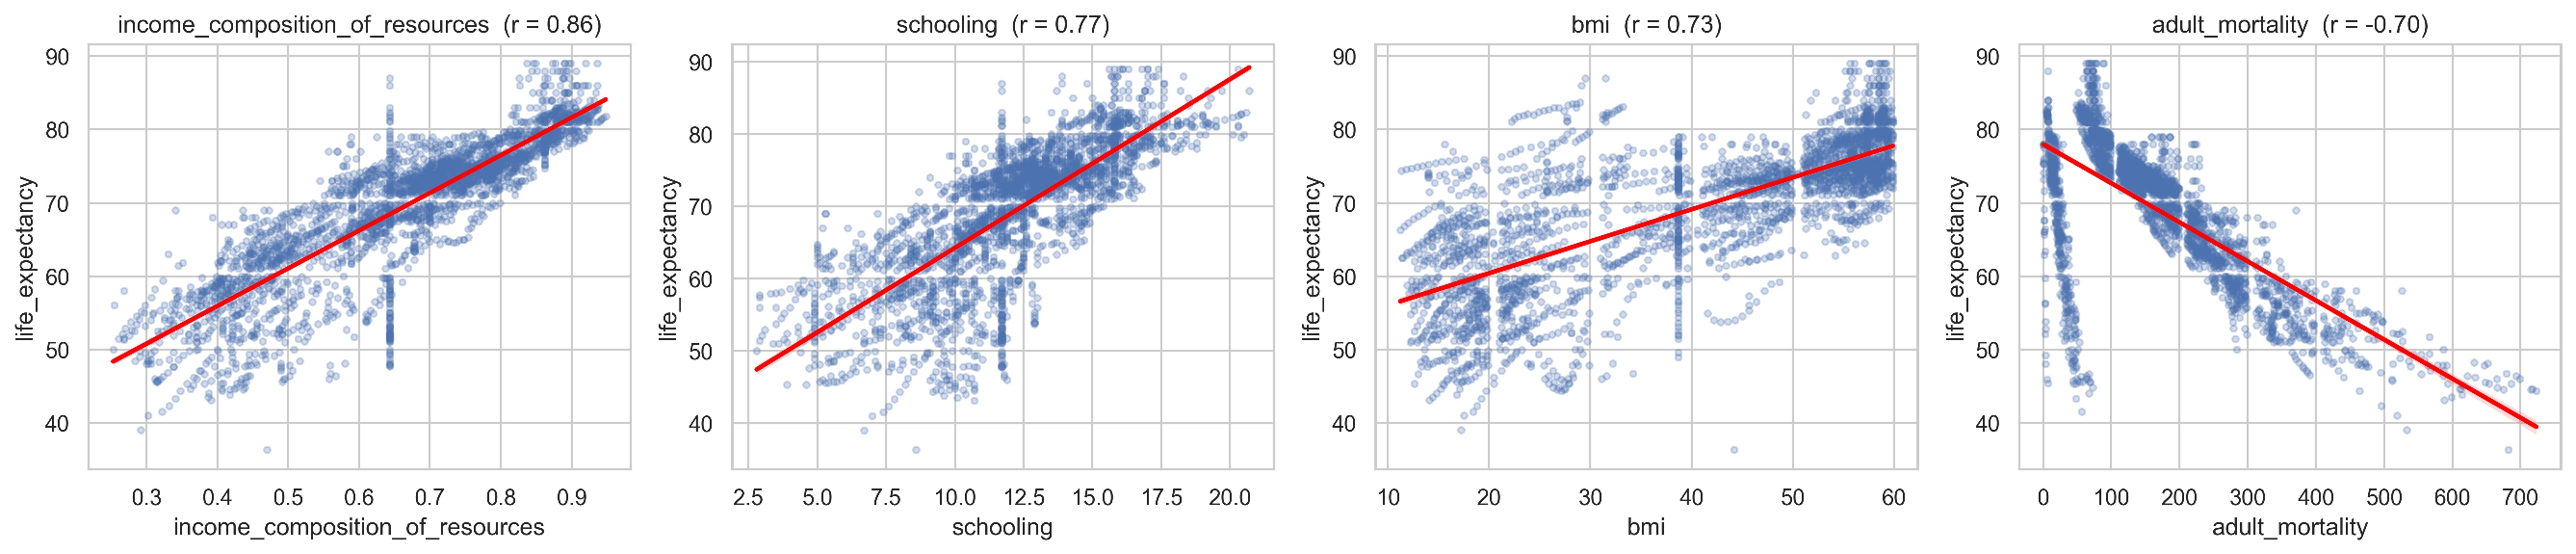
\includegraphics[width=\textwidth]{figs/scatter_top4.pdf}
\caption{The four features most correlated with life expectancy (with linear trend line).}
\end{figure}
The four strongest linear relationships are \texttt{income\_composition\_of\_resources}
($r=0.86$), \texttt{schooling} ($r=0.77$), \texttt{bmi} ($r=0.73$) and
\texttt{adult\_mortality} ($r=-0.70$). Higher resource-composition and schooling go together with
longer lives, while higher adult mortality goes with shorter lives.

\begin{figure}[H]\centering
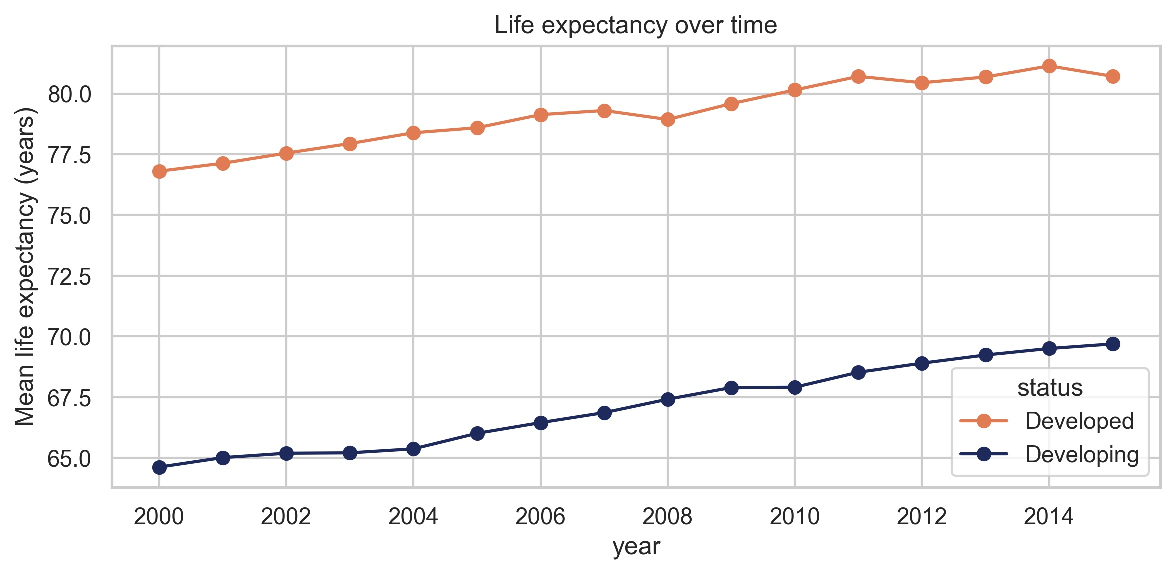
\includegraphics[width=0.7\textwidth]{figs/trend_by_year.pdf}
\caption{Mean life expectancy by year and development status.}
\end{figure}
Life expectancy rose in both groups between 2000 and 2015. Developed countries increased from
76.80 to 80.71 years (+3.91), while Developing countries increased from 64.62 to 69.69 years
(+5.07), so the gap narrowed from 12.18 to 11.02 years.

\begin{figure}[H]\centering
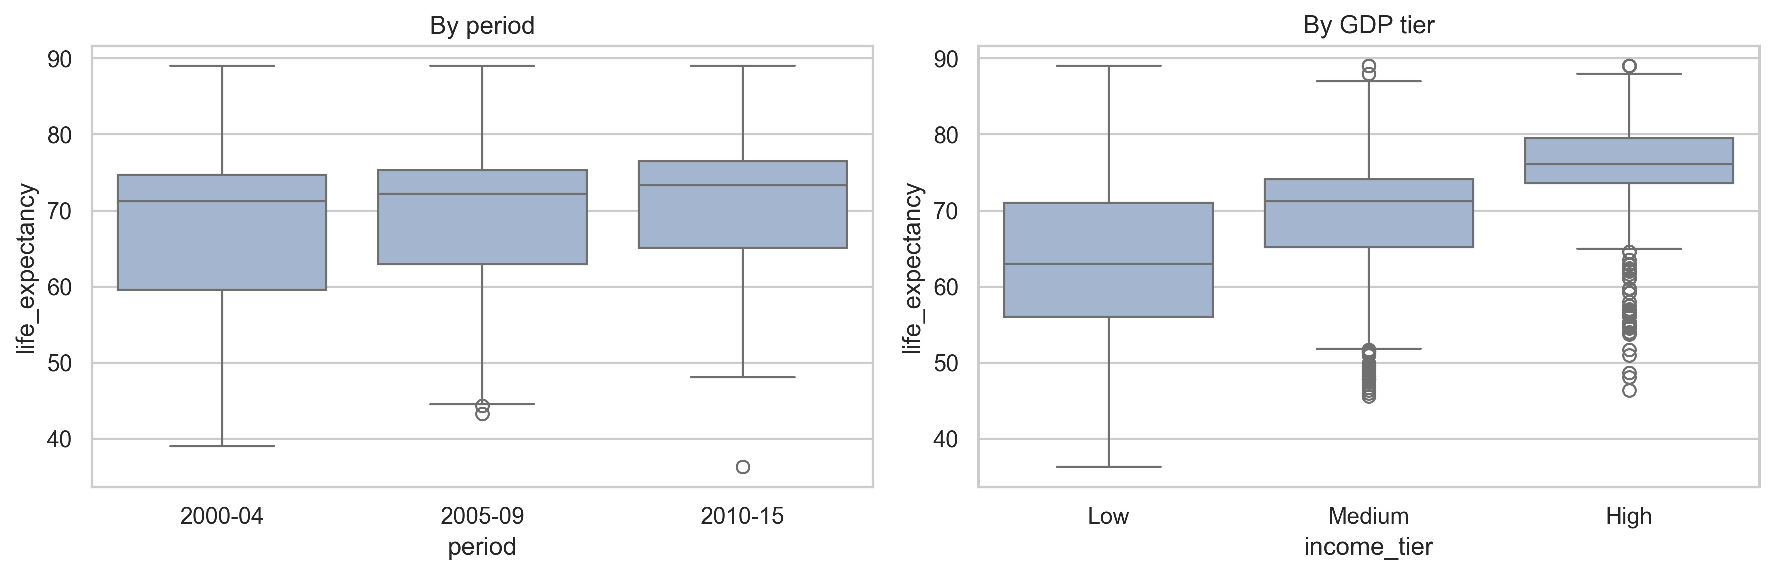
\includegraphics[width=\textwidth]{figs/categorical_vs_target.pdf}
\caption{Life expectancy by period (left) and GDP tier (right).}
\end{figure}
Mean life expectancy increases with GDP tier: 62.75 years (Low), 68.98 (Medium) and 75.95 (High),
and with time: 67.26 (2000--04), 69.06 (2005--09) and 71.00 (2010--15). The group differences are
statistically significant: Welch $t=47.87$ for status ($p<0.001$), ANOVA $F=39.70$ for period
($p<0.001$) and $F=691.15$ for GDP tier ($p<0.001$). \texttt{status} and \texttt{income\_tier} are also
strongly associated with each other ($\chi^2=592.75$, 2 df, $p<0.001$), so the two carry
overlapping information.

\subsection{Correlation Analysis}
\begin{figure}[H]\centering
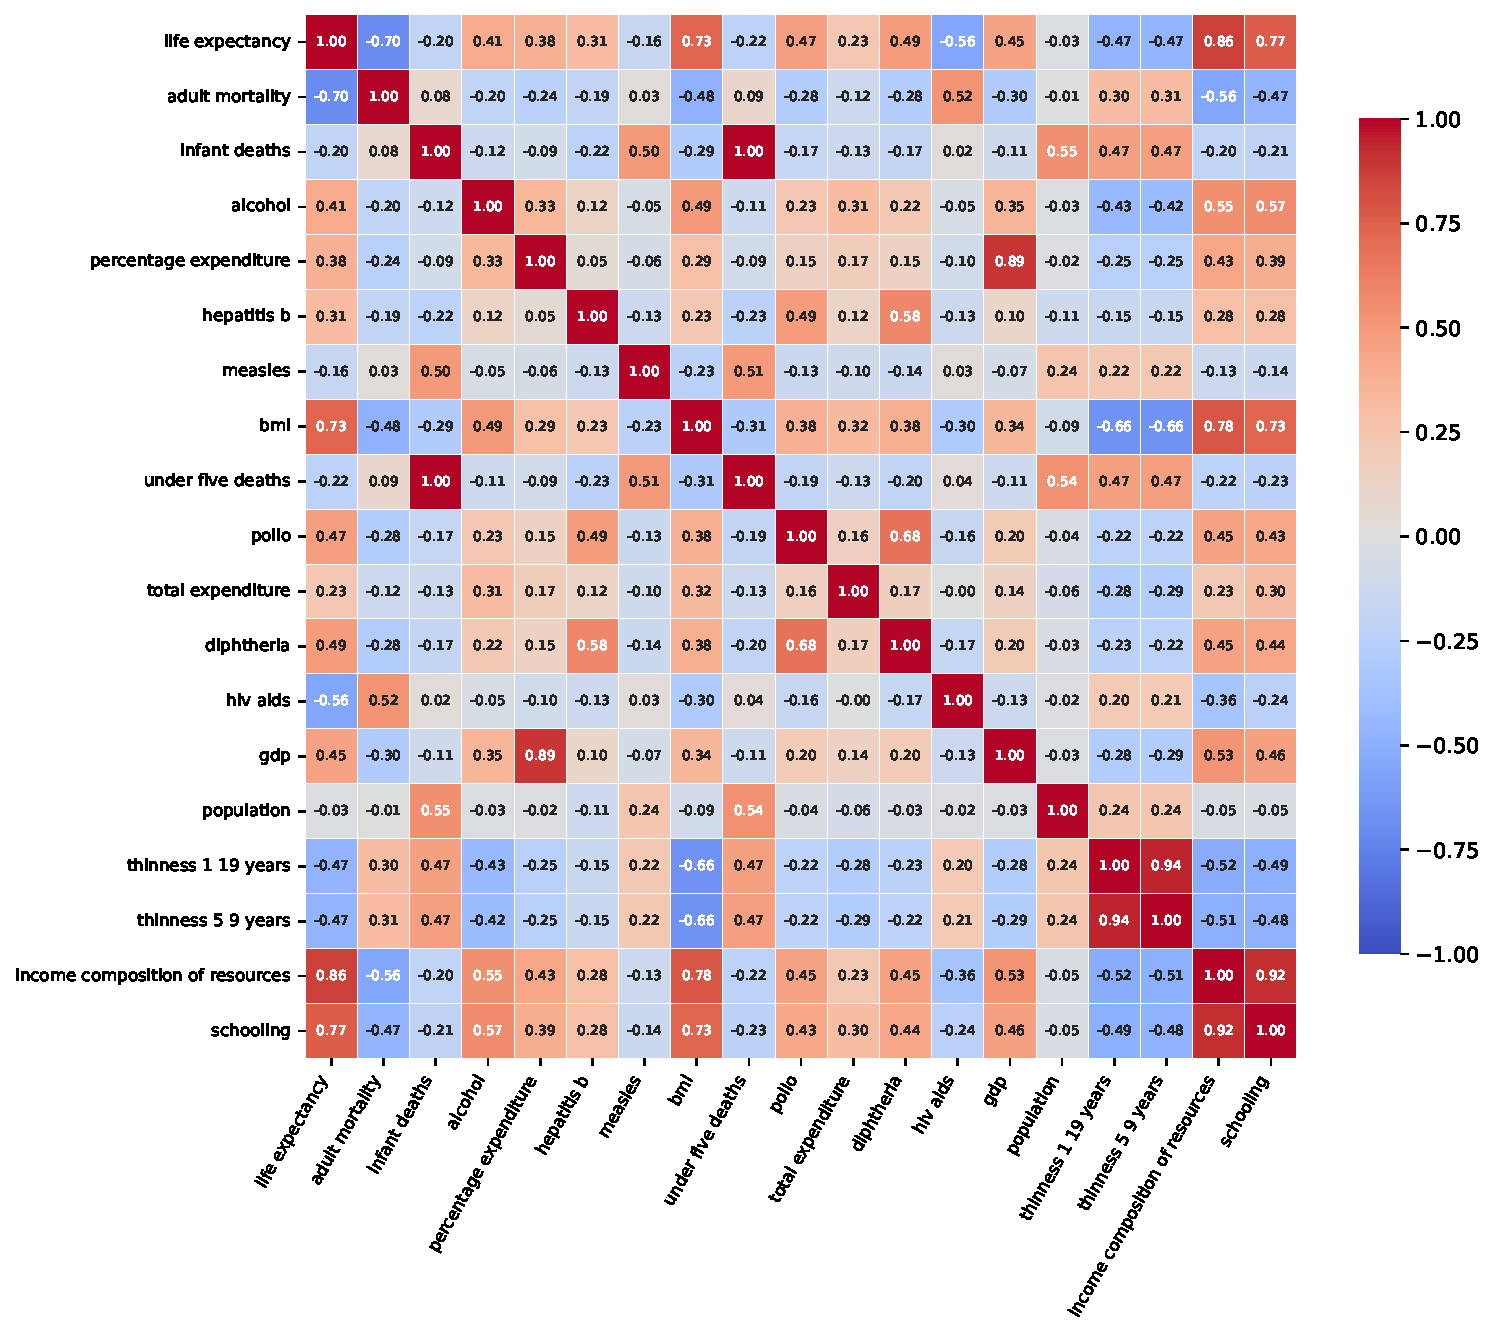
\includegraphics[width=1\textwidth]{figs/pearson_heatmap.pdf}
\caption{Pearson correlation matrix of the numeric features (after cleaning).}
\end{figure}

\begin{table}[H]\centering
\caption{Correlation of selected features with life expectancy (ordered by $|$Pearson$|$).}
\begin{tabular}{lrr}\toprule
\textbf{Feature} & \textbf{Pearson} & \textbf{Spearman}\\\midrule
income\_composition\_of\_resources & 0.861 & 0.883\\
schooling & 0.765 & 0.809\\
bmi & 0.727 & 0.740\\
adult\_mortality & $-0.696$ & $-0.650$\\
hiv\_aids & $-0.557$ & $-0.754$\\
diphtheria & 0.485 & 0.549\\
thinness\_1\_19\_years & $-0.472$ & $-0.609$\\
polio & 0.472 & 0.539\\
gdp & 0.448 & 0.630\\
under\_five\_deaths & $-0.222$ & $-0.616$\\
infant\_deaths & $-0.197$ & $-0.599$\\
population & $-0.029$ & $-0.088$\\\bottomrule
\end{tabular}\end{table}

\textbf{Non-linear relationships.} Spearman correlations are much larger than Pearson for
\texttt{infant\_deaths} ($-0.20$ vs.\ $-0.60$), \texttt{under\_five\_deaths} ($-0.22$ vs.\ $-0.62$),
\texttt{hiv\_aids} ($-0.56$ vs.\ $-0.75$) and \texttt{gdp} (0.45 vs.\ 0.63). These variables are
related to life expectancy in a monotonic but non-linear way, which suggests that non-linear models
may fit better than a straight line.

\textbf{Multicollinearity.} Several predictors are almost duplicates of each other:
\begin{table}[H]\centering
\caption{Predictor pairs with $|r|>0.7$.}
\begin{tabular}{llr}\toprule
\textbf{Feature 1} & \textbf{Feature 2} & \textbf{$|r|$}\\\midrule
infant\_deaths & under\_five\_deaths & 0.997\\
thinness\_1\_19\_years & thinness\_5\_9\_years & 0.939\\
income\_composition\_of\_resources & schooling & 0.919\\
percentage\_expenditure & gdp & 0.893\\
bmi & income\_composition\_of\_resources & 0.783\\
bmi & schooling & 0.727\\\bottomrule
\end{tabular}\end{table}

\subsection{EDA Hypotheses}
\begin{itemize}
\item $H_1$: Higher schooling is associated with higher life expectancy.
      \emph{Supported:} $r=0.77$ (Spearman 0.81).
\item $H_2$: Developed countries have significantly higher life expectancy.
      \emph{Supported:} 79.20 vs.\ 67.11 years, a difference of 12.09 years
      (Welch $t=47.87$, $p<0.001$).
\item $H_3$: Adult mortality has a strong negative effect.
      \emph{Supported:} $r=-0.70$ (Spearman $-0.65$); \texttt{hiv\_aids} is also strongly negative
      ($r=-0.56$, Spearman $-0.75$).
\end{itemize}

%==================== IV. MODEL DEVELOPMENT ====================
\section{Model Development}\label{sec:model}
\subsection{Model Selection}
The target is a continuous variable, so supervised regression was used. Four models were compared
against a baseline that always predicts the training mean:
\begin{itemize}
  \item \textbf{Linear Regression:} an interpretable parametric reference model.
  \item \textbf{Ridge Regression:} linear regression with an L2 penalty, chosen because several
        predictors are strongly correlated (see the correlation pairs table and the VIF table below).
  \item \textbf{Random Forest:} an ensemble of 300 trees that captures non-linear effects and
        interactions.
  \item \textbf{Gradient Boosting:} sequential trees that each correct the previous errors; the
        non-linear relationships found in the EDA make it a natural candidate.
\end{itemize}

\subsection{Feature Selection}
Eighteen features were used: \texttt{adult\_mortality}, \texttt{infant\_deaths}, \texttt{alcohol},
\texttt{percentage\_expenditure}, \texttt{hepatitis\_b}, \texttt{measles}, \texttt{bmi},
\texttt{polio}, \texttt{total\_expenditure}, \texttt{diphtheria}, \texttt{hiv\_aids}, \texttt{gdp},
\texttt{population}, \texttt{thinness\_1\_19\_years}, \texttt{income\_composition\_of\_resources},
\texttt{schooling}, \texttt{year} and \texttt{status}. From each near-duplicate pair, one variable
was dropped: \texttt{under\_five\_deaths} ($r=0.997$ with \texttt{infant\_deaths}) and
\texttt{thinness\_5\_9\_years} ($r=0.939$ with \texttt{thinness\_1\_19\_years}).

\begin{table}[H]\centering
\caption{Variance inflation factors of the largest features (training set).}
\begin{tabular}{lr}\toprule
\textbf{Feature} & \textbf{VIF}\\\midrule
income\_composition\_of\_resources & 12.57\\
schooling & 7.56\\
bmi & 3.33\\
infant\_deaths & 3.04\\
gdp & 2.82\\
diphtheria & 2.43\\\bottomrule
\end{tabular}\end{table}
Only \texttt{income\_composition\_of\_resources} exceeds the common threshold of 10, and all
remaining features not shown in the table are below 2.5. Both it and \texttt{schooling} were kept, since they are of
substantive interest and Ridge and tree models tolerate collinearity, but their coefficients must
be interpreted together.

\newpage

\subsection{Splitting and Scaling}
The data was split 80/20 \emph{by country} (\texttt{GroupShuffleSplit}, \texttt{random\_state=42}),
so that the same country never appears in both sets. This avoids leakage, since the rows of one
country are very similar across years. The training set has 2336 rows (146 countries) and the test
set 592 rows (37 countries). \texttt{StandardScaler} was fitted on the training set only and applied
to both sets, for all features except the binary \texttt{status}.
\begin{lstlisting}
gss = GroupShuffleSplit(n_splits=1, test_size=0.2, random_state=42)
train_idx, test_idx = next(gss.split(X, y, groups))
scaler = StandardScaler().fit(X_train[scale_cols])   # fit on train only
\end{lstlisting}

\subsection{Baseline and Training}
The baseline predicts the training mean for every country-year (test RMSE 9.95 years). Linear and
Ridge Regression used default settings (Ridge with the tuned $\alpha$), Random Forest used 300 trees,
and Gradient Boosting used the \texttt{scikit-learn} defaults, all with \texttt{random\_state=42}.
Each model was also evaluated with 5-fold grouped cross-validation (\texttt{GroupKFold}) on the
training set.

\subsection{Hyperparameter Tuning}
The Ridge penalty $\alpha$ was tuned with 5-fold grouped cross-validation over seven values.
\begin{lstlisting}
GridSearchCV(Ridge(), {"alpha": [0.001, 0.01, 0.1, 1, 10, 100, 1000]},
             cv=GroupKFold(n_splits=5), scoring="neg_root_mean_squared_error")
\end{lstlisting}
\begin{table}[H]\centering
\caption{Ridge tuning results (mean CV RMSE and its standard deviation across folds).}
\begin{tabular}{rcc}\toprule
\textbf{$\alpha$} & \textbf{CV RMSE} & \textbf{Std}\\\midrule
0.001 & 3.6538 & 0.498\\
0.01 & 3.6538 & 0.498\\
0.1 & 3.6538 & 0.498\\
1 & 3.6533 & 0.497\\
\textbf{10} & \textbf{3.6499} & 0.488\\
100 & 3.6519 & 0.448\\
1000 & 3.8558 & 0.447\\\bottomrule
\end{tabular}\end{table}
The best value was $\alpha=10$ (CV RMSE 3.6499). The differences between $\alpha\le 100$ are tiny,
and only a very strong penalty ($\alpha=1000$) hurts. Random Forest and Gradient Boosting were not tuned.

%==================== V. RESULTS ====================
\section{Results and Evaluation}
\subsection{Model Comparison}
\begin{table}[H]\centering
\caption{Model performance (grouped split by country; CV = 5-fold grouped cross-validation on the training set).}
\begin{tabular}{lccccc}\toprule
\textbf{Model} & \textbf{Train RMSE} & \textbf{CV RMSE} & \textbf{Test RMSE} & \textbf{Test MAE} & \textbf{Test $R^2$}\\\midrule
Baseline (mean) & 9.4262 & -- & 9.9487 & 7.9821 & $-0.0593$\\
Linear Regression & 3.3686 & 3.6538 & 3.2422 & 2.5075 & 0.8875\\
Ridge (tuned) & 3.3692 & 3.6499 & 3.2426 & 2.5029 & 0.8875\\
Random Forest & 0.6373 & 2.9956 & 2.6476 & 1.9300 & 0.9250\\
Gradient Boosting & 1.8457 & 3.0064 & \textbf{2.5890} & 1.9495 & \textbf{0.9283}\\\bottomrule
\end{tabular}\end{table}

\begin{figure}[H]\centering
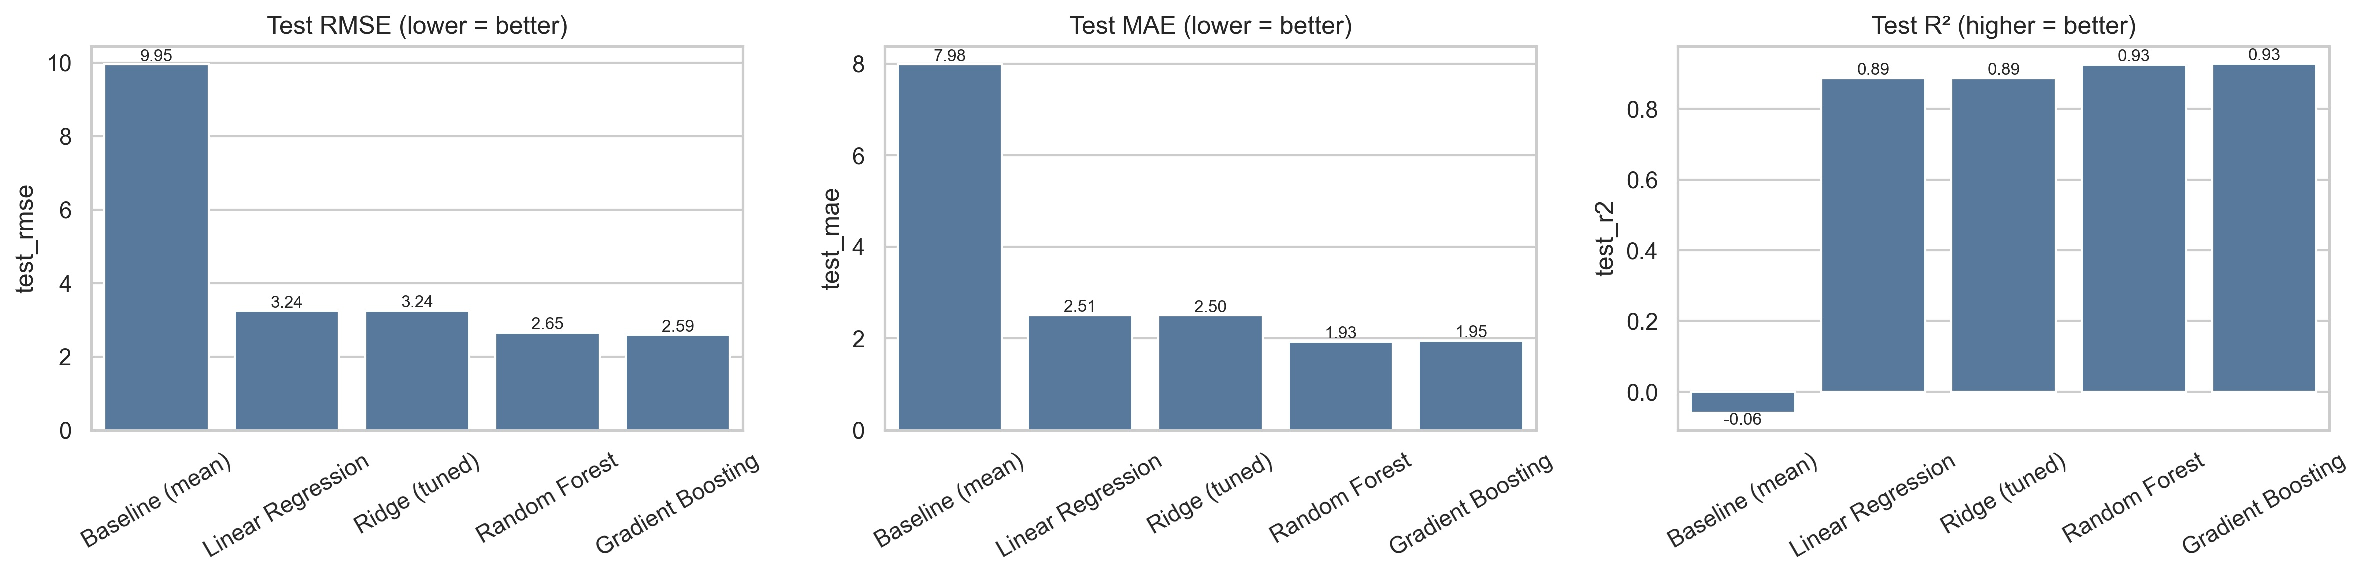
\includegraphics[width=\textwidth]{figs/model_comparison.pdf}
\caption{Test RMSE, MAE and $R^2$ across models.}
\end{figure}

\textbf{Key observations.}
\begin{itemize}
  \item \textbf{All models beat the baseline.} Predicting the training mean gives a test
        RMSE of 9.95 years. Gradient Boosting reduces this to 2.59 years (a 74\% reduction)
        and explains 92.8\% of the variance in life expectancy of unseen countries.
        The baseline $R^2$ is slightly negative ($-0.06$) because the test countries
        have a different mean than the training countries.
  \item \textbf{Ridge matches Linear Regression.} Their results differ by less than
        0.001 in RMSE, so regularization changes almost nothing here.
  \item \textbf{Tree ensembles outperform linear models.} Gradient Boosting lowers
        the test RMSE by about 20\% relative to Linear Regression (2.59 vs.\ 3.24) and
        improves $R^2$ from 0.888 to 0.928. The CV RMSE shows the same gap
        (about 3.0 vs.\ 3.65), which suggests the relationships are partly non-linear, consistent
        with the larger Spearman than Pearson correlations found in the EDA
        (e.g.\ \texttt{hiv\_aids}, \texttt{infant\_deaths}).
  \item \textbf{Random Forest overfits more than Gradient Boosting.} Its training RMSE is
        0.64, far below its CV RMSE of 3.00, while Gradient Boosting's training
        RMSE is 1.85 against a CV RMSE of 3.01.
  \item \textbf{Gradient Boosting and Random Forest perform almost equally.}
        Gradient Boosting has the lowest test RMSE, but the gap to Random Forest is only 0.06 years
        and Random Forest has a slightly lower CV RMSE, so neither can be called clearly better.
        Gradient Boosting is selected as the best model by test RMSE.
  \item \textbf{Test error is lower than CV error for every model.} The test set contains only
        37 countries, so a single split can be easier or harder than average; the CV RMSE is the more
        conservative estimate.
  \item \textbf{Practical accuracy.} The best model's MAE is 1.95 years, so its predictions are
        typically within about two years of the actual value, compared with a standard
        deviation of 9.52 years in the target.
\end{itemize}

\subsection{Predicted vs.\ Actual and Residuals}
\begin{figure}[H]\centering
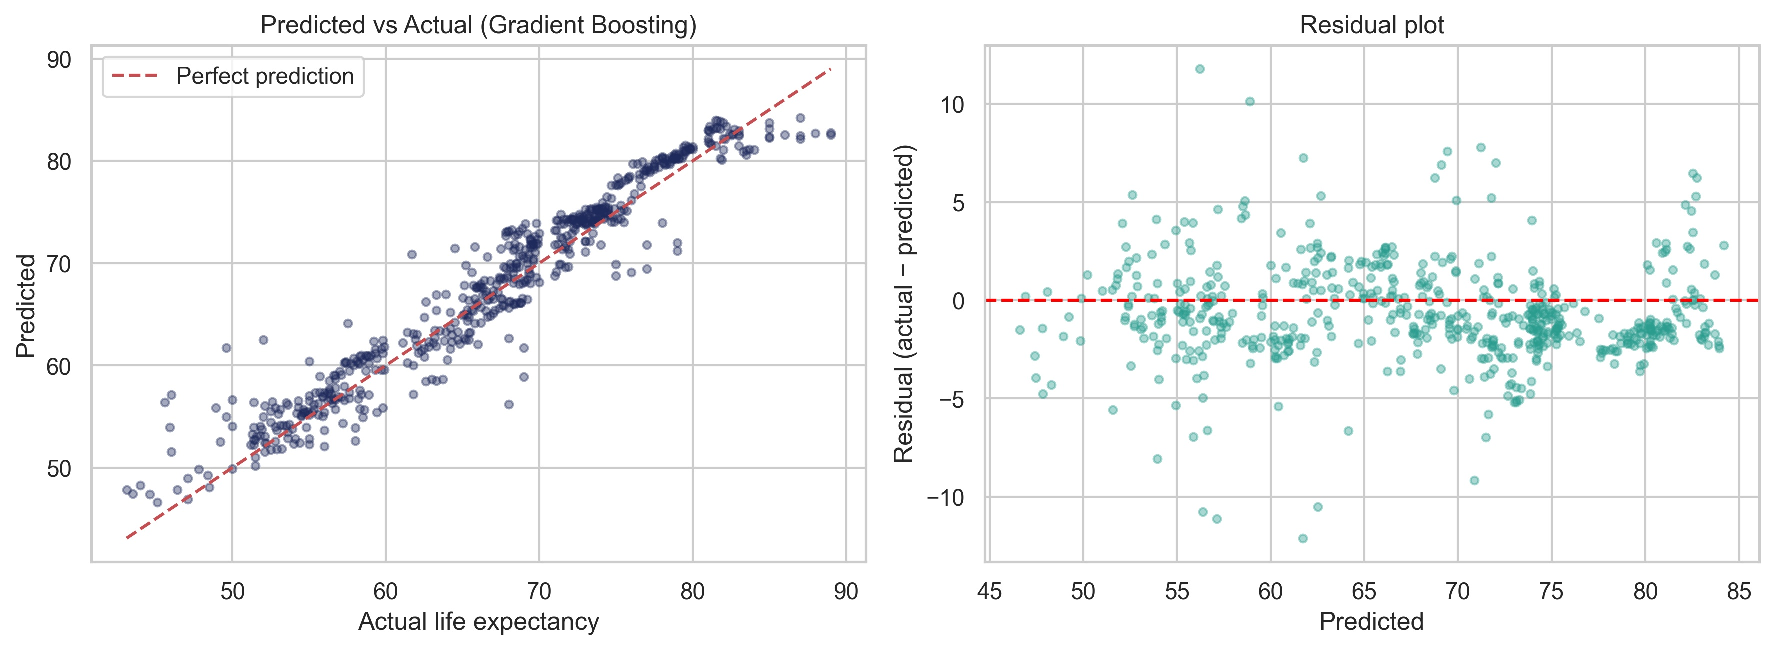
\includegraphics[width=\textwidth]{figs/pred_vs_actual_residuals.pdf}
\caption{Gradient Boosting: predicted vs.\ actual life expectancy (left) and residuals (right) on the test set.}
\end{figure}
The predictions follow the diagonal closely over the whole range. The model slightly
over-predicts the lowest values (below about 50 years) and under-predicts the highest values
(above about 82 years), since predictions flatten at the extremes where there are few countries.
The mean residual is $-0.71$ years (a slight tendency to over-predict) with a standard deviation
of 2.49 years. Most residuals lie within $\pm 5$ years, with a few errors of up to about 12 years.
The residuals show no strong trend against the predicted value, although clusters of similar
errors suggest that some individual countries are consistently mis-predicted.

\subsection{Feature Importance and Coefficients}
\begin{figure}[H]\centering
\begin{subfigure}{0.48\textwidth}\centering
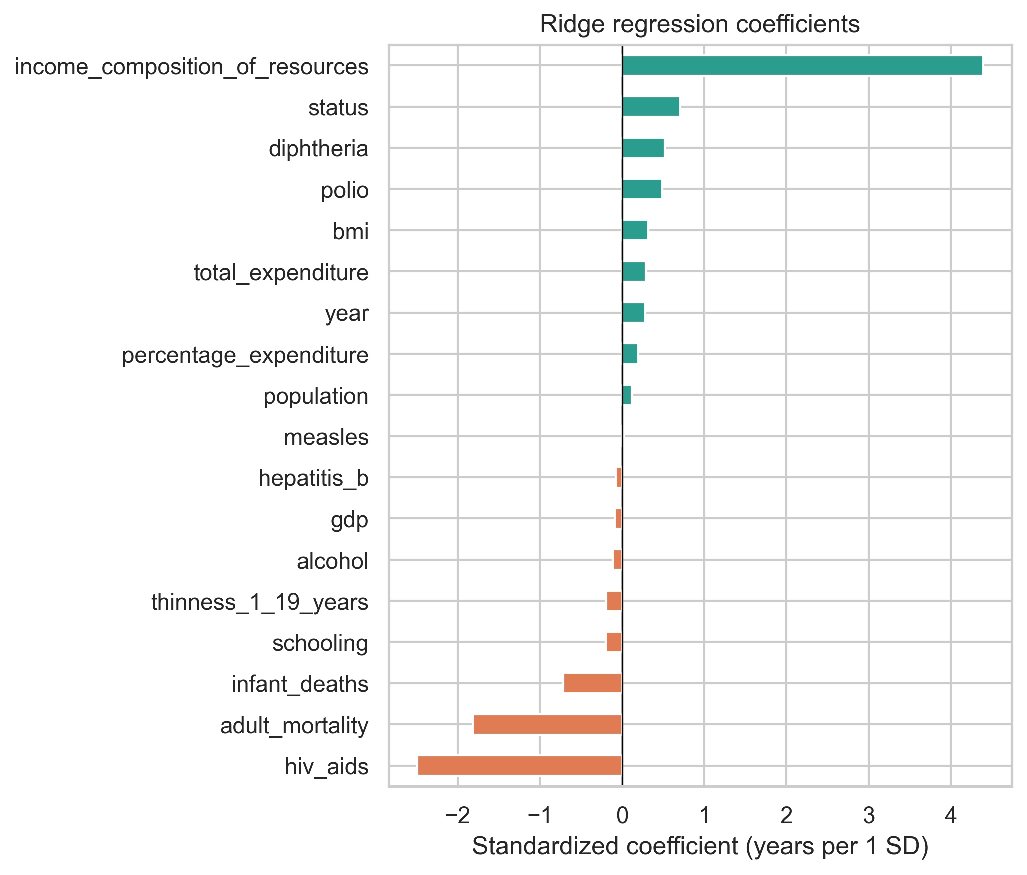
\includegraphics[width=\textwidth]{figs/ridge_coefficients.pdf}
\caption{Ridge standardized coefficients.}
\end{subfigure}\hfill
\begin{subfigure}{0.48\textwidth}\centering
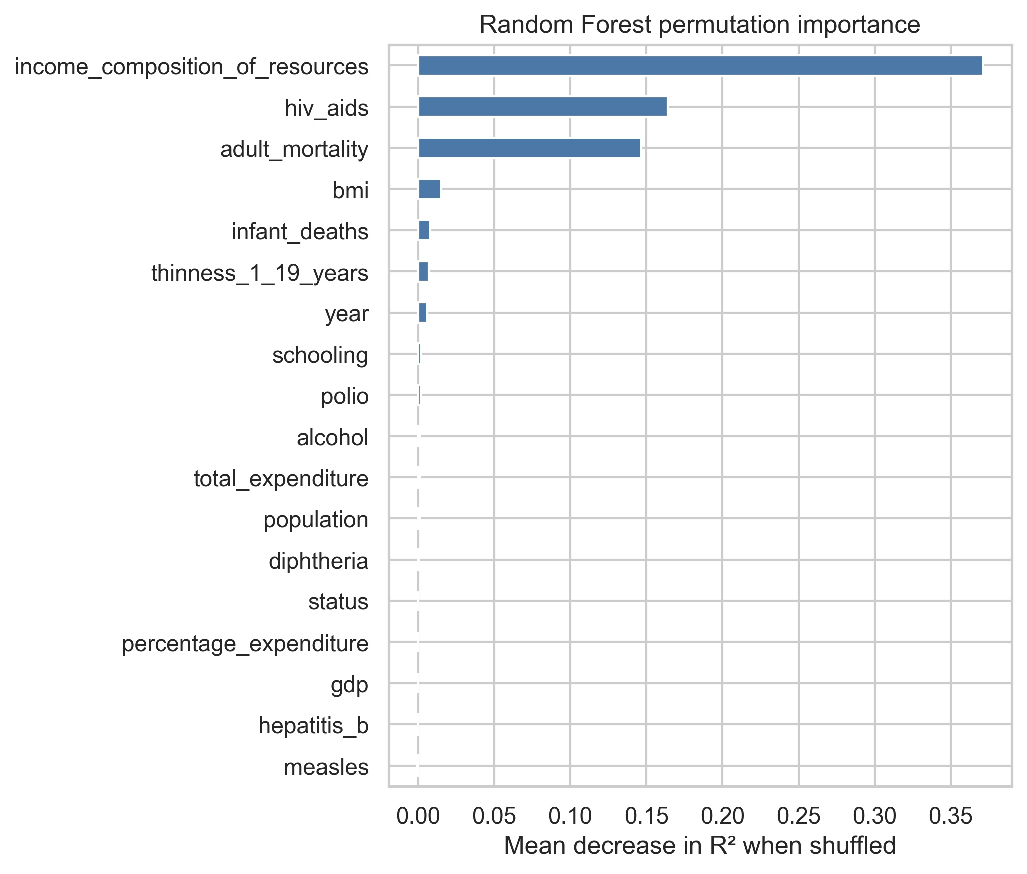
\includegraphics[width=\textwidth]{figs/rf_permutation_importance.pdf}
\caption{Random Forest permutation importance.}
\end{subfigure}
\caption{Feature importance from a linear and a non-linear model.}
\end{figure}

\textbf{Ridge coefficients} (years of life expectancy per one standard deviation for scaled predictors
--- on the $\log(1+x)$ scale for log-transformed features --- or for Developed vs.\ Developing for
binary \texttt{status}, other features held constant) show that \texttt{income\_composition\_of\_resources}
is by far the strongest positive effect ($+4.40$), followed by \texttt{status} (Developed, $+0.71$),
\texttt{diphtheria} ($+0.52$) and \texttt{polio} ($+0.49$). The strongest negative effects are
\texttt{hiv\_aids} ($-2.49$), \texttt{adult\_mortality} ($-1.82$) and \texttt{infant\_deaths} ($-0.71$).

\textbf{Random Forest permutation importance} (drop in test $R^2$ when a feature is shuffled)
agrees on the top three: \texttt{income\_composition\_of\_resources} (0.371), \texttt{hiv\_aids} (0.164)
and \texttt{adult\_mortality} (0.147). The next features, \texttt{bmi} (0.015) and
\texttt{infant\_deaths} (0.008), are an order of magnitude smaller, and most remaining features
contribute almost nothing once these are known.

\textbf{Schooling.} Although \texttt{schooling} is strongly correlated with life expectancy
($r=0.77$), its Ridge coefficient is slightly negative ($-0.20$) and its permutation importance is
small (0.002). This is not evidence that education is harmful: \texttt{schooling} and
\texttt{income\_composition\_of\_resources} are highly correlated ($r=0.92$, VIF 12.6), so the model
attributes their shared effect to the latter. The two variables should therefore be interpreted
together, and $H_1$ is supported by the correlation analysis rather than by the model coefficient.

\begin{table}[H]\centering
\caption{Summary of the EDA hypotheses.}
\begin{tabularx}{\textwidth}{lXl}\toprule
\textbf{Hypothesis} & \textbf{Evidence} & \textbf{Result}\\\midrule
$H_1:$ schooling $\uparrow$, life expectancy $\uparrow$ & $r=0.77$; overlaps with income composition in the models & Supported\\
$H_2:$ Developed $>$ Developing & 12.09 years higher; Ridge coefficient $+0.71$ after controlling for other features & Supported\\
$H_3:$ adult mortality $\downarrow$ life expectancy & $r=-0.70$; Ridge $-1.82$; third in permutation importance & Supported\\\bottomrule
\end{tabularx}\end{table}

%==================== VI. CONCLUSION ====================
\section{Conclusion and Business Implications}
\subsection{Key Findings}
\begin{enumerate}
  \item \textbf{Life expectancy can be predicted accurately.} Gradient Boosting reached a test RMSE
        of 2.59 years, MAE of 1.95 years and $R^2=0.928$, a 74\% reduction in error compared with
        predicting the mean (RMSE 9.95).
  \item \textbf{Non-linear models fit better.} Tree ensembles beat Linear and Ridge Regression
        (test RMSE 2.59--2.65 vs.\ 3.24), in line with the non-linear patterns seen in the EDA.
  \item \textbf{The main drivers are resource development and mortality.}
        Income composition of resources ($r=0.86$) is the dominant predictor in both
        Ridge and Random Forest, followed by \texttt{hiv\_aids} and \texttt{adult\_mortality},
        both strongly negative.
  \item \textbf{A large development gap exists but is narrowing.} Developed countries live 12.09
        years longer on average; the gap shrank from 12.18 years in 2000 to 11.02 in 2015 because
        Developing countries improved faster (+5.07 vs.\ +3.91 years).
  \item \textbf{Schooling and income composition overlap.} Schooling is strongly related to
        longevity, but most of its effect is shared with income composition ($r=0.92$), so the
        two cannot be separated reliably.
\end{enumerate}

\subsection{Implications}
\begin{itemize}
  \item \textbf{Health ministries and development agencies:} the results point to reducing HIV/AIDS
        and adult mortality, and to improving the broader economic and educational conditions
        summarized by the resource-composition index, as the most promising levers.
  \item \textbf{International organizations (e.g.\ WHO):} the model can estimate life expectancy
        for countries with incomplete data and identify countries whose actual value is far from the
        prediction, which may deserve closer investigation.
  \item \textbf{Funders and NGOs:} the narrowing gap suggests that investment in Developing
        countries is paying off, while the remaining 11-year gap shows where need is greatest.
\end{itemize}

\subsection{Limitations}
\begin{itemize}
  \item \textbf{Imputation:} \texttt{population} is missing for 22\% of rows (48 countries entirely)
        and \texttt{gdp} for 15\%; the status median used for such countries is a rough estimate.
  \item \textbf{Data quality:} 629 \texttt{bmi} values were implausible, and the remaining
        values should be treated with caution. \texttt{percentage\_expenditure} and
        \texttt{measles} contain values that conflict with their documented units.
  \item \textbf{Ecological data:} the observations are country-level averages, so the results do
        not describe individuals, and correlation does not imply causation.
  \item \textbf{Possible overlap of \texttt{income\_composition\_of\_resources} with the target:}
        its definition is not fully documented; if it partly encodes health outcomes, its
        importance may be overstated.
  \item \textbf{Evaluation:} results rely on a single country-based split with only 37 test countries,
        and Random Forest and Gradient Boosting were not tuned.
\end{itemize}

\subsection{Future Work}
\begin{itemize}
  \item Tune Random Forest and Gradient Boosting and repeat the grouped split several times to
        obtain confidence intervals.
  \item Use panel or mixed-effects models that exploit the country-year structure and model time trends.
  \item Replace imputation with external, more complete sources for GDP and population, and use
        more recent data than 2015.
  \item Test the sensitivity of the results to removing \texttt{bmi} and to dropping either
        \texttt{schooling} or \texttt{income\_composition\_of\_resources}.
\end{itemize}


%==================== REFERENCES (APA 7) ====================
\clearpage
\phantomsection
\addcontentsline{toc}{section}{References}
\begin{center}
  {\Large\bfseries References}
\end{center}
\vspace{0.4cm}

{\begingroup
\raggedright
\setlength{\parindent}{-0.5in}
\setlength{\leftskip}{0.5in}
\setlength{\parskip}{6pt}

Breiman, L. (2001). Random forests. \emph{Machine Learning}, \emph{45}(1), 5--32. \url{https://doi.org/10.1023/A:1010933404324}

Friedman, J.\ H. (2001). Greedy function approximation: A gradient boosting machine. \emph{The Annals of Statistics}, \emph{29}(5), 1189--1232. \url{https://doi.org/10.1214/aos/1013203451}

Harris, C.\ R., Millman, K.\ J., van der Walt, S.\ J., Gommers, R., Virtanen, P., Cournapeau, D., Wieser, E., Taylor, J., Berg, S., Smith, N.\ J., Kern, R., Picus, M., Hoyer, S., van Kerkwijk, M.\ H., Brett, M., Haldane, A., Fern\'andez del R\'io, J., Wiebe, M., Peterson, P., \ldots\ Oliphant, T.\ E. (2020). Array programming with NumPy. \emph{Nature}, \emph{585}(7825), 357--362. \url{https://doi.org/10.1038/s41586-020-2649-2}

Hoerl, A.\ E., \& Kennard, R.\ W. (1970). Ridge regression: Biased estimation for nonorthogonal problems. \emph{Technometrics}, \emph{12}(1), 55--67. \url{https://doi.org/10.1080/00401706.1970.10488634}

Hunter, J.\ D. (2007). Matplotlib: A 2D graphics environment. \emph{Computing in Science \& Engineering}, \emph{9}(3), 90--95. \url{https://doi.org/10.1109/MCSE.2007.55}

McKinney, W. (2010). Data structures for statistical computing in Python. In S.\ van der Walt \& J.\ Millman (Eds.), \emph{Proceedings of the 9th Python in Science Conference} (pp.\ 56--61). \url{https://doi.org/10.25080/Majora-92bf1922-00a}

Pedregosa, F., Varoquaux, G., Gramfort, A., Michel, V., Thirion, B., Grisel, O., Blondel, M., Prettenhofer, P., Weiss, R., Dubourg, V., Vanderplas, J., Passos, A., Cournapeau, D., Brucher, M., Perrot, M., \& Duchesnay, \'E. (2011). Scikit-learn: Machine learning in Python. \emph{Journal of Machine Learning Research}, \emph{12}(85), 2825--2830. \url{https://jmlr.org/papers/v12/pedregosa11a.html}

Rajarshi, K. (n.d.). \emph{Life Expectancy (WHO)} [Data set]. Kaggle. \url{https://www.kaggle.com/datasets/kumarajarshi/life-expectancy-who}

Virtanen, P., Gommers, R., Oliphant, T.\ E., Haberland, M., Reddy, T., Cournapeau, D., Burovski, E., Peterson, P., Weckesser, W., Bright, J., van der Walt, S.\ J., Brett, M., Wilson, J., Millman, K.\ J., Mayorov, N., Nelson, A.\ R.\ J., Jones, E., Kern, R., Larson, E., \ldots\ SciPy 1.0 Contributors. (2020). SciPy 1.0: Fundamental algorithms for scientific computing in Python. \emph{Nature Methods}, \emph{17}(3), 261--272. \url{https://doi.org/10.1038/s41592-019-0686-2}

Waskom, M.\ L. (2021). seaborn: Statistical data visualization. \emph{Journal of Open Source Software}, \emph{6}(60), Article 3021. \url{https://doi.org/10.21105/joss.03021}

World Health Organization. (n.d.). \emph{Global Health Observatory data repository} [Data set]. \url{https://www.who.int/data/gho}

\par\endgroup}

%==================== APPENDICES (APA 7) ====================
\clearpage
\phantomsection
\addcontentsline{toc}{section}{Appendix A: Source Code and Dataset Access}
\begin{center}
  {\Large\bfseries Appendix A}\\[4pt]
  {\large\bfseries Source Code and Dataset Access}
\end{center}
\vspace{0.3cm}

The complete Jupyter notebook (\texttt{life\_expectancy\_analysis.ipynb}), exported CSV summary tables, generated figures, LaTeX report source, and presentation slides are publicly available for reproducibility:
\begin{itemize}
  \item \textbf{Source code repository:} \url{https://github.com/5H31BYYY/Data_Analysis_I_Final}
  \item \textbf{Original dataset (Kaggle):} \url{https://www.kaggle.com/datasets/kumarajarshi/life-expectancy-who}
\end{itemize}

\clearpage
\phantomsection
\addcontentsline{toc}{section}{Appendix B: Data Dictionary and Raw Data Sample}
\begin{center}
  {\Large\bfseries Appendix B}\\[4pt]
  {\large\bfseries Data Dictionary and Raw Data Sample}
\end{center}
\vspace{0.3cm}

\renewcommand{\thetable}{B\arabic{table}}
\setcounter{table}{0}

\refstepcounter{table}\label{tab:dict}
\noindent\textbf{Table \thetable}\\
\emph{Data Dictionary of Cleaned and Engineered Variables}

\vspace{4pt}
{\singlespacing\footnotesize\renewcommand{\arraystretch}{1.18}
\noindent\begin{tabularx}{\textwidth}{l l X}\toprule
\textbf{Variable} & \textbf{Type} & \textbf{Description}\\\midrule
\texttt{country} & Qualitative & Country name\\
\texttt{year} & Ordinal & Year of observation (2000--2015)\\
\texttt{status} & Qualitative & Development status (Developed or Developing)\\
\texttt{life\_expectancy} & Quantitative (target) & Life expectancy at birth, in years\\
\texttt{adult\_mortality} & Quantitative & Adult mortality rate, both sexes, per 1,000 population\\
\texttt{infant\_deaths} & Quantitative & Number of infant deaths per 1,000 population\\
\texttt{alcohol} & Quantitative & Alcohol consumption per capita, in litres of pure alcohol\\
\texttt{percentage\_expenditure} & Quantitative & Health expenditure as \% of GDP per capita\\
\texttt{hepatitis\_b} & Quantitative & Hepatitis B immunization coverage (\%)\\
\texttt{measles} & Quantitative & Reported measles cases per 1,000 population\\
\texttt{bmi} & Quantitative & Average body mass index of the population\\
\texttt{under\_five\_deaths} & Quantitative & Deaths under age five per 1,000 population\\
\texttt{polio} & Quantitative & Polio immunization coverage (\%)\\
\texttt{total\_expenditure} & Quantitative & Government health expenditure as \% of total government expenditure\\
\texttt{diphtheria} & Quantitative & Diphtheria (DTP3) immunization coverage (\%)\\
\texttt{hiv\_aids} & Quantitative & Deaths per 1,000 live births due to HIV/AIDS, ages 0--4\\
\texttt{gdp} & Quantitative & Gross domestic product per capita, in USD\\
\texttt{population} & Quantitative & Total population of the country\\
\texttt{thinness\_1\_19\_years} & Quantitative & Prevalence of thinness among ages 10--19 (\%)\\
\texttt{thinness\_5\_9\_years} & Quantitative & Prevalence of thinness among ages 5--9 (\%)\\
\texttt{income\_composition\_of\_resources} & Quantitative & Human Development Index in terms of income composition (0--1)\\
\texttt{schooling} & Quantitative & Average years of schooling\\
\texttt{period} & Qualitative (engineered) & Year grouped into 2000--04, 2005--09, and 2010--15 (EDA only)\\
\texttt{income\_tier} & Qualitative (engineered) & GDP per capita tertile: Low, Medium, High (EDA only)\\\bottomrule
\end{tabularx}\par}
\vspace{4pt}
\noindent{\small\emph{Note.} All column names were standardized to snake\_case during preprocessing. \texttt{period} and \texttt{income\_tier} were engineered for exploratory analysis only and excluded from regression modeling.}

\vspace{0.7cm}

\noindent\begin{minipage}{\textwidth}
\refstepcounter{table}\label{tab:rawsample}
\noindent\textbf{Table \thetable}\\
\emph{Sample of the Raw Dataset (First Five Observations, Selected Columns)}
\vspace{4pt}
\begin{center}
\singlespacing\small
\begin{tabular}{lcclccr}\toprule
\textbf{Country} & \textbf{Year} & \textbf{Status} & \textbf{Life exp.} & \textbf{Adult mort.} & \textbf{Schooling} & \textbf{Income comp.}\\\midrule
Afghanistan & 2015 & Developing & 65.0 & 263 & 10.1 & 0.479\\
Afghanistan & 2014 & Developing & 59.9 & 271 & 10.0 & 0.476\\
Afghanistan & 2013 & Developing & 59.9 & 268 & 9.9 & 0.470\\
Afghanistan & 2012 & Developing & 59.5 & 272 & 9.8 & 0.463\\
Afghanistan & 2011 & Developing & 59.2 & 275 & 9.5 & 0.454\\\bottomrule
\end{tabular}
\end{center}
\vspace{2pt}
\noindent{\small\emph{Note.} Adapted from \emph{Life Expectancy (WHO)} [Data set], by K.\ Rajarshi, n.d., Kaggle (\url{https://www.kaggle.com/datasets/kumarajarshi/life-expectancy-who}). Life exp.\ = life expectancy (years); Adult mort.\ = adult mortality per 1,000 population; Income comp.\ = income composition of resources.}
\end{minipage}

\clearpage
\phantomsection
\addcontentsline{toc}{section}{Appendix C: Supplementary Exploratory Figures}
\begin{center}
  {\Large\bfseries Appendix C}\\[4pt]
  {\large\bfseries Supplementary Exploratory Figures}
\end{center}
\vspace{0.3cm}

\renewcommand{\thefigure}{C\arabic{figure}}
\setcounter{figure}{0}

\begin{figure}[H]
\refstepcounter{figure}\label{fig:hist}
\noindent\textbf{Figure \thefigure}\\
\emph{Histograms of Numeric Predictors After Cleaning}\par
\vspace{6pt}
{\centering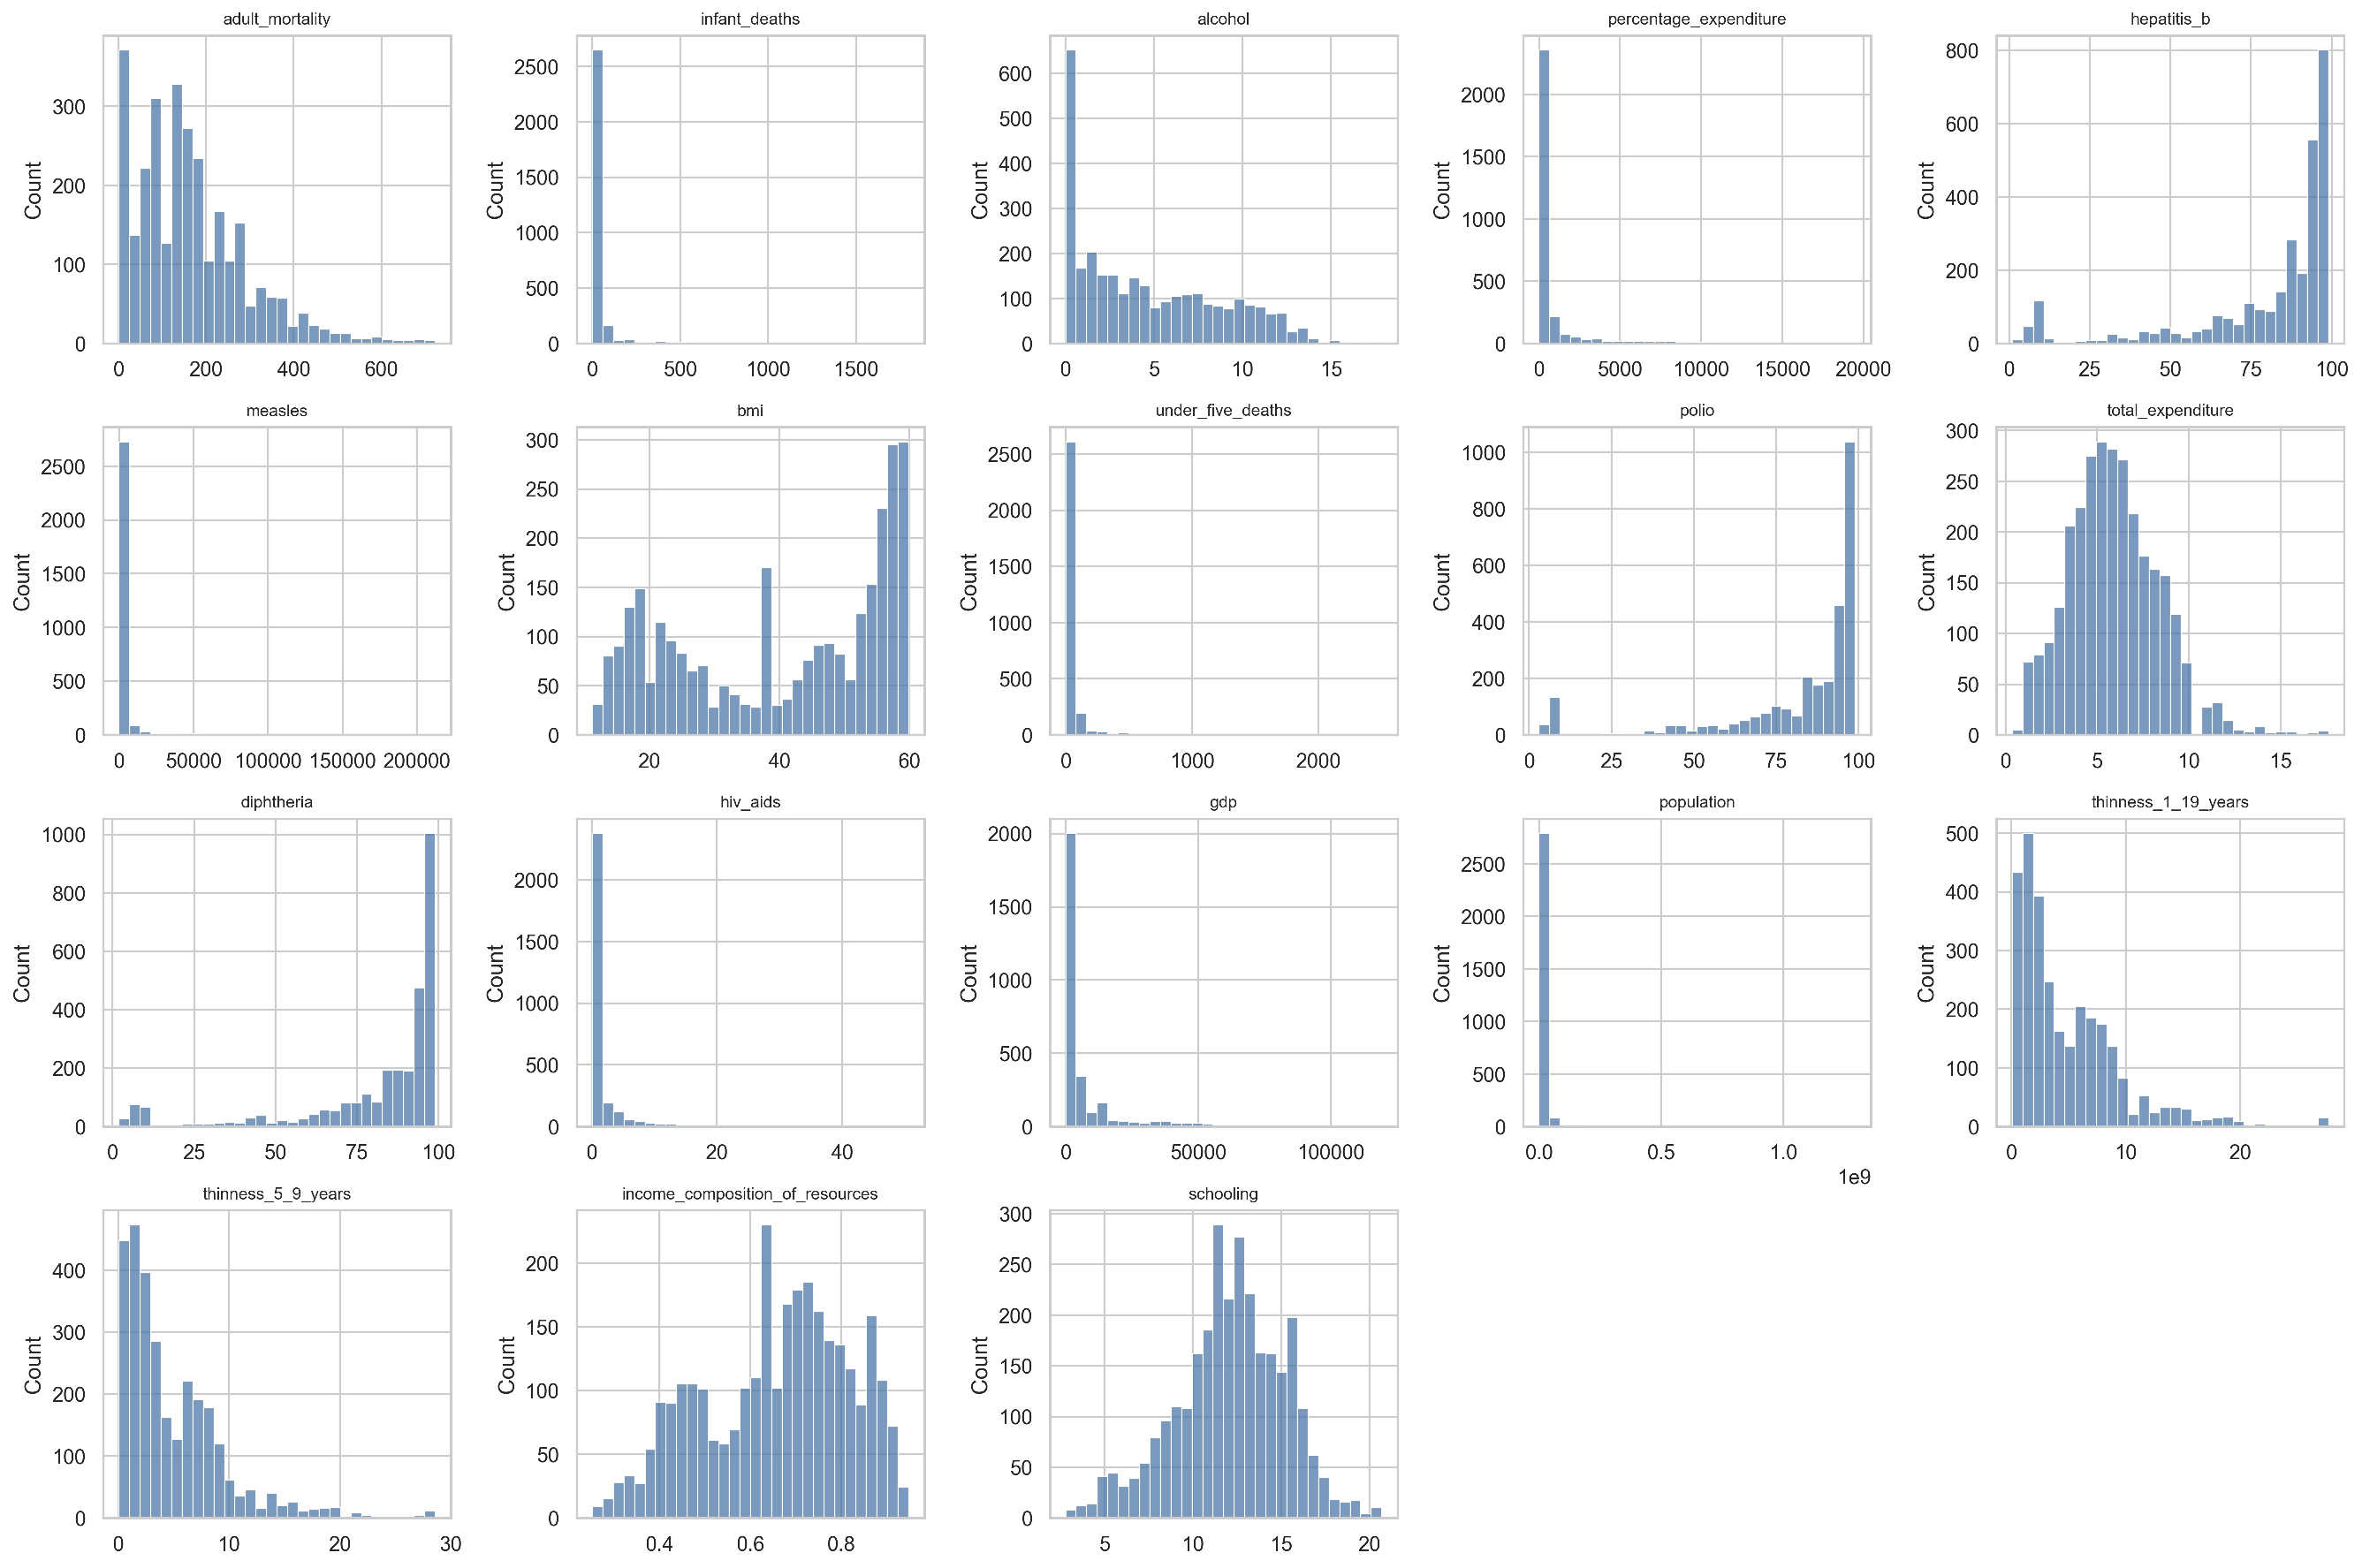
\includegraphics[width=\textwidth]{figs/histograms_numeric.pdf}\par}
\vspace{4pt}
\noindent{\small\emph{Note.} Distributions of the 18 numeric predictors after invalid-value replacement and median imputation (excluding \texttt{year} and the target variable \texttt{life\_expectancy}).}
\end{figure}

\vspace{0.6cm}

\begin{figure}[H]
\refstepcounter{figure}\label{fig:boxplots}
\noindent\textbf{Figure \thefigure}\\
\emph{Boxplots of Numeric Features After Cleaning}\par
\vspace{6pt}
{\centering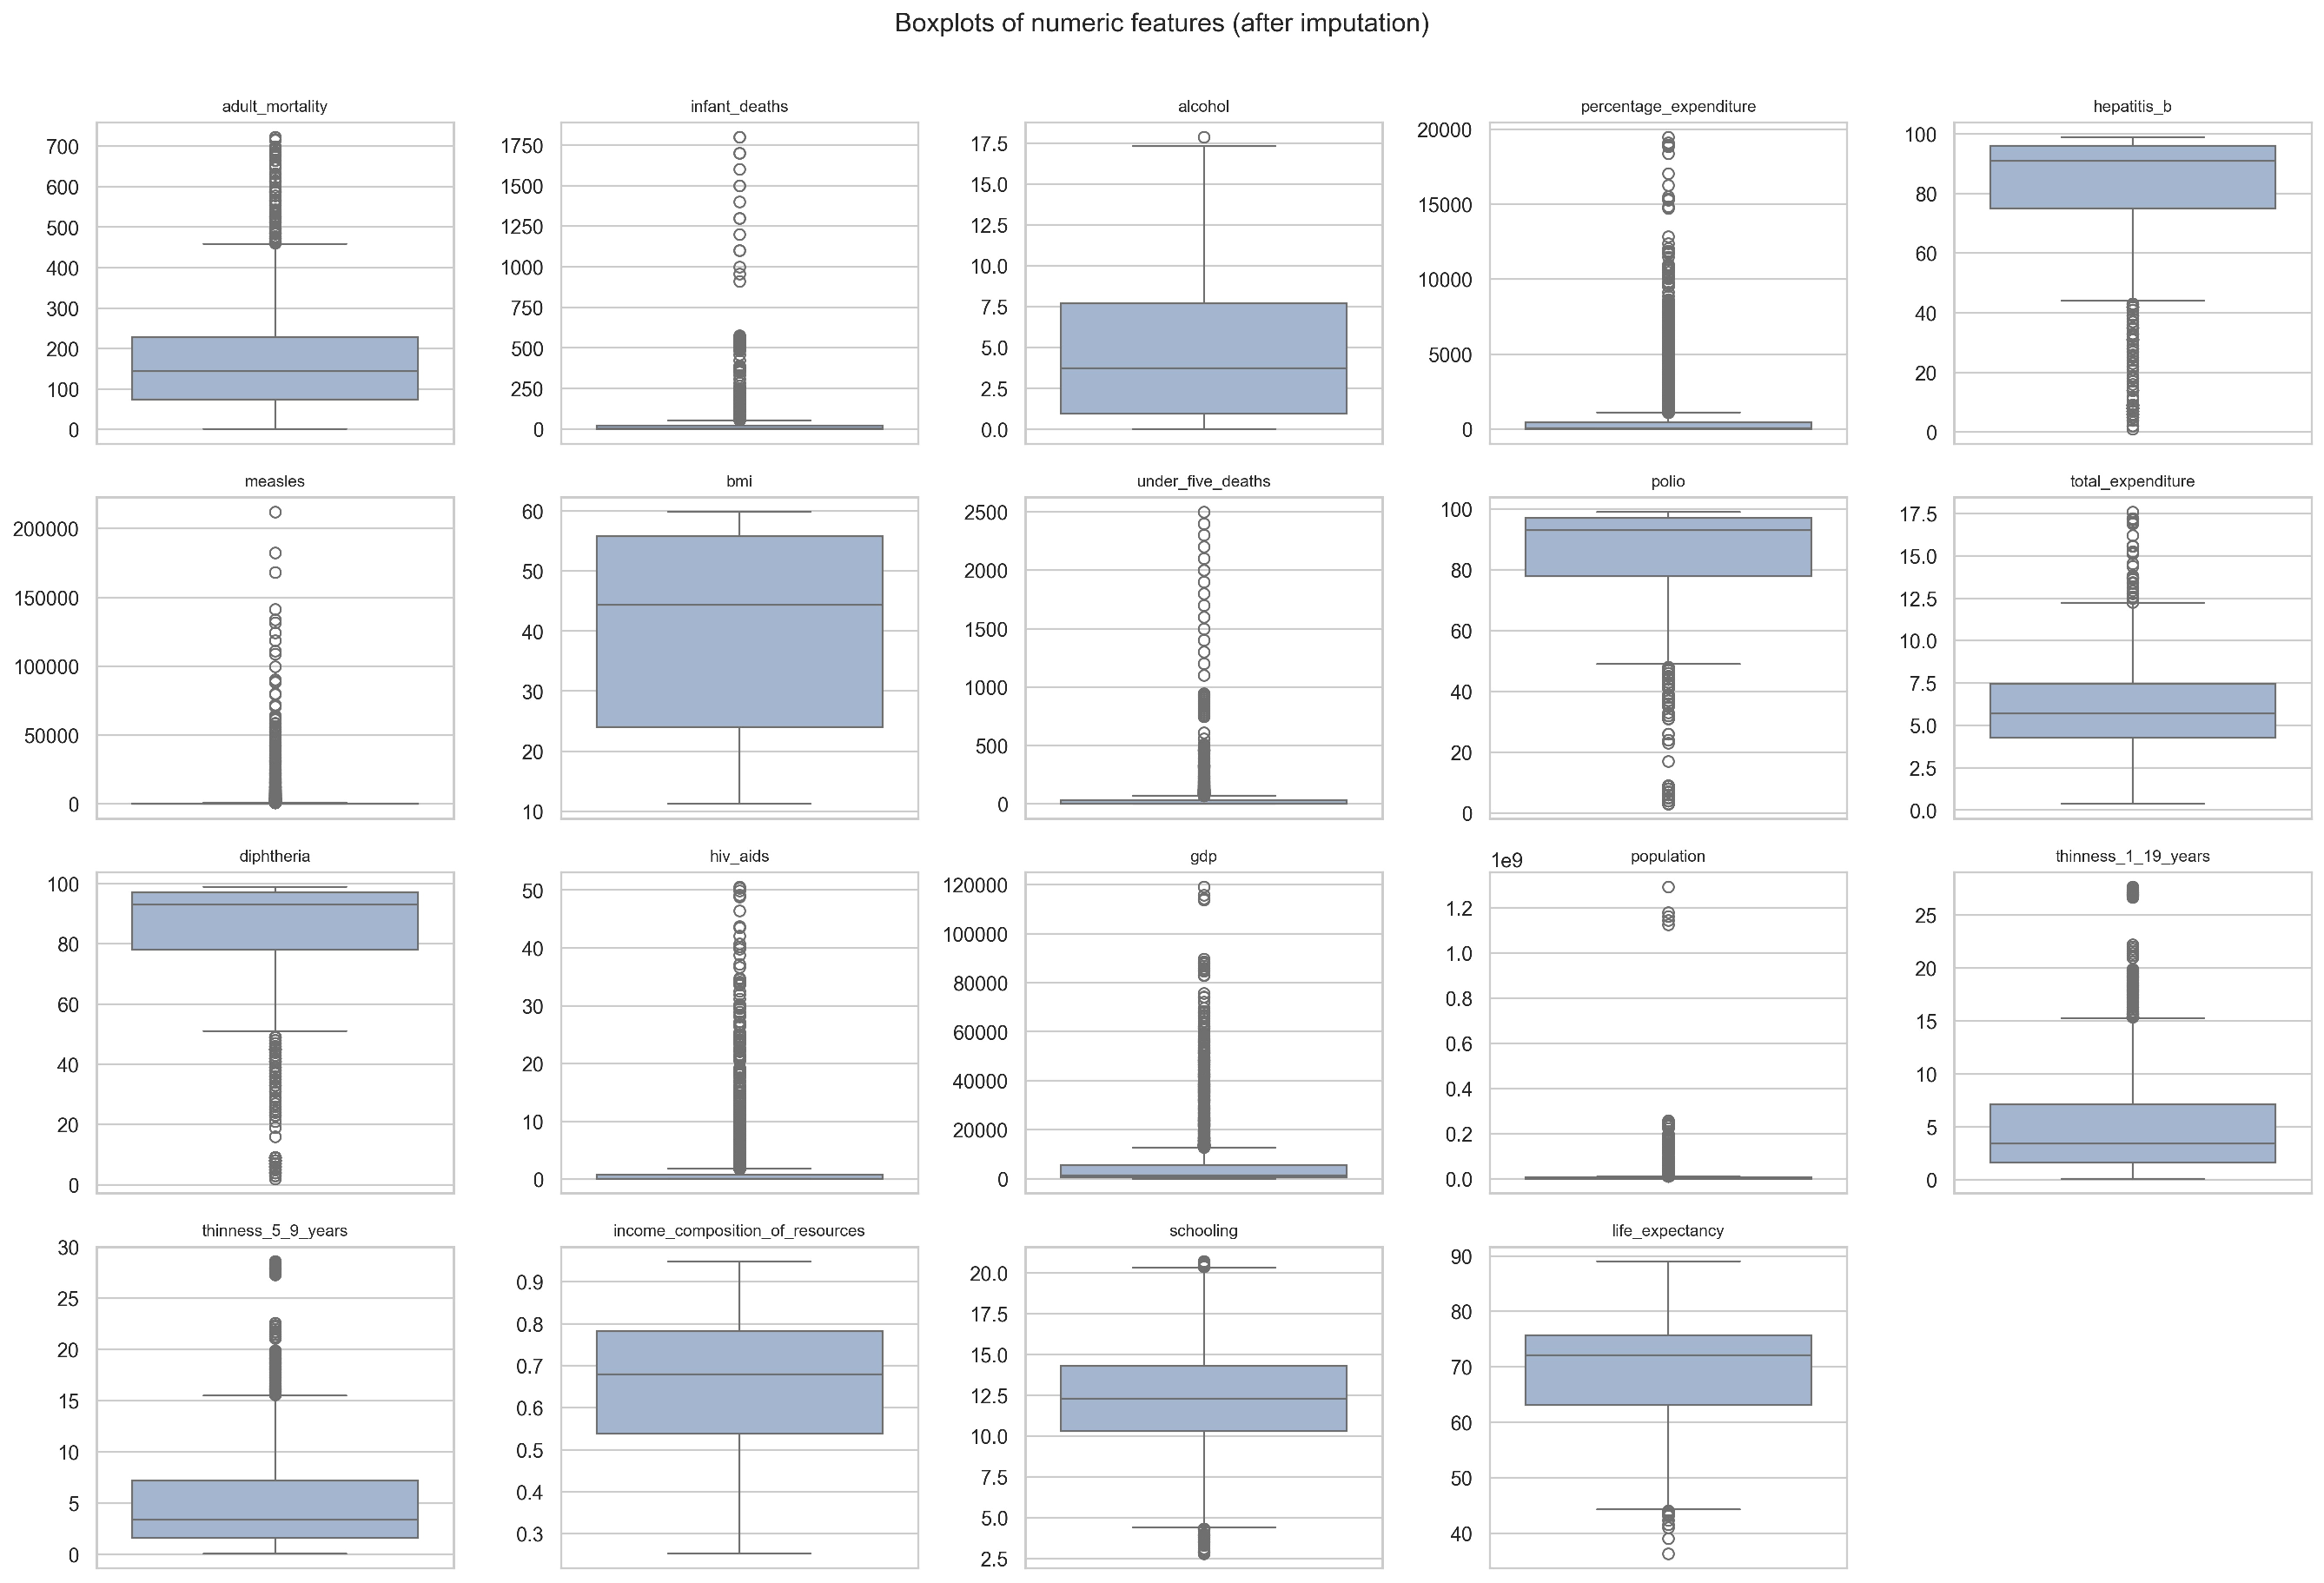
\includegraphics[width=\textwidth]{figs/boxplots_numeric.pdf}\par}
\vspace{4pt}
\noindent{\small\emph{Note.} Boxplots of the 18 numeric predictors and target variable \texttt{life\_expectancy} after imputation (excluding \texttt{year}), illustrating right-skewed distributions with genuine extreme observations.}
\end{figure}

\end{document}